%==============================================================================
\chapter{Spontaniteit van processen}
\label{ch:spontaniteit}
%==============================================================================

\section{Waarom spontaniteit? De warmtepomp}
\label{sec:energie-en-richting}

Nieuwe woningen krijgen steeds vaker geen gasaansluiting meer, en de warmtepomp vervangt de gasketel. Zo'n toestel haalt warmte uit de buitenlucht, ook als het buiten maar \SI{5}{\celsius} is, en pompt die naar een woning van \SI{20}{\celsius} (figuur~\ref{fig:warmtepomp}). Een koelmiddel verdampt in de buitenunit bij een temperatuur onder die van de buitenlucht en neemt daarbij warmte op. Een compressor perst de damp samen, waardoor ze heter wordt dan het water van de vloerverwarming (hoofdstuk~\ref{ch:energie}, \S\ref{sec:compressor}). In de condensor geeft de damp haar warmte af en condenseert ze. Via een ventiel gaat de vloeistof terug naar buiten. Een koelkast, een airco en de koelmachine van de ammoniakfabriek werken precies zo.

\begin{figure}[htb]
    \centering
    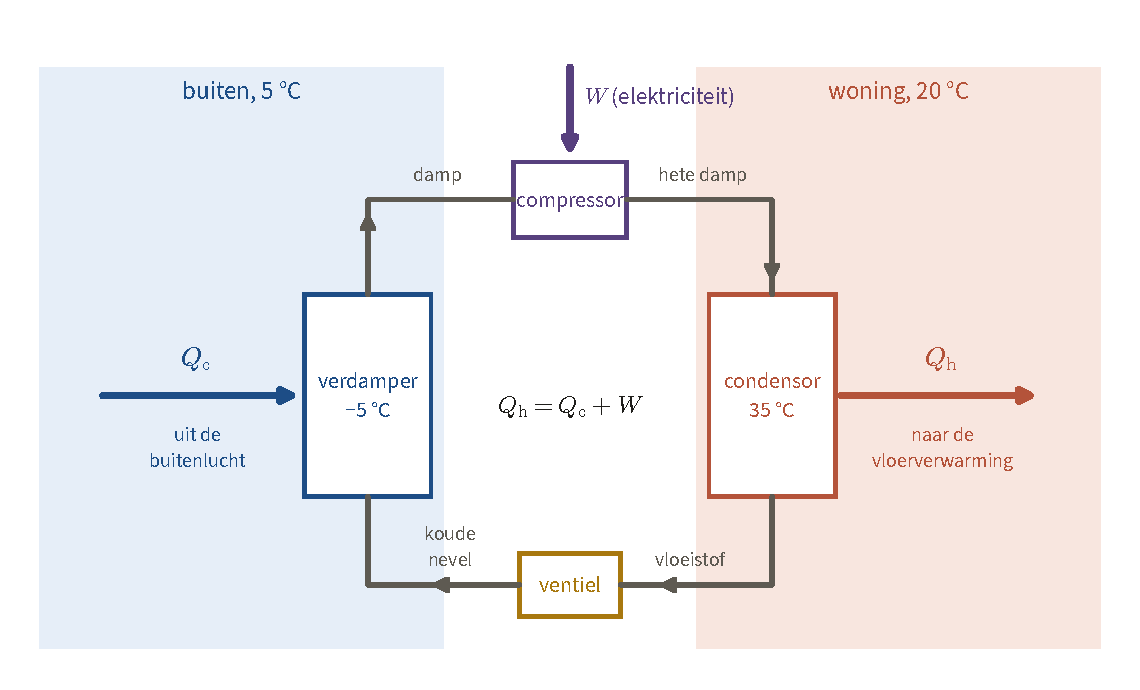
\includegraphics[width=0.85\linewidth]{Figuren/warmtepomp_schema}
    \caption{Kringloop van een lucht-waterwarmtepomp. Het koelmiddel neemt warmte $Q_\mathrm{c}$ op uit de koude buitenlucht, de compressor voegt arbeid $W$ toe, en de condensor geeft $Q_\mathrm{h} = Q_\mathrm{c} + W$ af aan de vloerverwarming.}
    \label{fig:warmtepomp}
\end{figure}

De eerste hoofdwet zegt enkel dat de energie klopt: $Q_\mathrm{h} = Q_\mathrm{c} + W$. Ze zegt niet waarom je de compressor nodig hebt. Waarom stroomt de warmte niet vanzelf van de buitenlucht naar binnen, zodat $W = 0$ volstaat? Dat soort vragen is het onderwerp van dit hoofdstuk:
\begin{itemize}
\item Waarom stroomt warmte vanzelf van warm naar koud, en nooit omgekeerd (\S\ref{sec:waarschijnlijkheid-entropie})?
\item Hoeveel elektriciteit heeft een warmtepomp minstens nodig per kilowattuur warmte, en waar hangt dat van af (\S\ref{sec:tweedehoofdwet})?
\item Is het dan beter om met een warmtepomp te verwarmen dan met een gasketel, die bijna alle energie van het gas als warmte afgeeft (\S\ref{sec:exergie})?
\item Bij welke temperatuur kookt het koelmiddel, en hoe kies je er een (\S\ref{sec:gibbs})?
\end{itemize}
Het antwoord vraagt een nieuwe grootheid, de \emph{entropie}. In hoofdstuk~\ref{ch:kwantum} zagen we dat energie over gekwantiseerde toestanden verdeeld wordt. Entropie telt op hoeveel manieren dat kan. Met de entropie volgt ook de grootheid die voor ingenieurs en chemici het belangrijkst is: de Gibbs-vrije energie, die zegt welke processen en reacties vanzelf verlopen. Net als in de vorige hoofdstukken start elke sectie met een probleem en werkt ze dat op het einde uit.

\section{Spontaniteit en de statistische oorsprong van entropie}

\begin{casus}{waarom stroomt warmte enkel van warm naar koud?}
Zet een warme kop koffie in een koude kamer en ze koelt af tot kamertemperatuur. Nooit warmt lauwe koffie zichzelf op door warmte uit de kamer te halen, hoewel de energie in beide richtingen behouden blijft. Waarom niet? Geen enkele kracht duwt de energie van warm naar koud.

\emph{Schat eerst zelf:} denk aan de energiekwanta van hoofdstuk~\ref{ch:kwantum}. Als je een handvol kwanta willekeurig verdeelt over de moleculen van twee voorwerpen, waar komen ze dan vooral terecht?
\end{casus}

Hete koffie die afkoelt, parfum dat zich door een kamer verspreidt, melk die zich mengt met koffie, een ijsblokje dat smelt in een warm drankje: het zijn heel verschillende processen, gedreven door warmteoverdracht, diffusie of een faseovergang. Toch hebben ze \'e\'en ding gemeen: ze verlopen vanzelf in \'e\'en richting, en nooit in de omgekeerde. Lauwe koffie warmt zichzelf nooit op, een mengsel ontmengt nooit vanzelf, en een glas water vormt nooit spontaan een ijsblokje op kamertemperatuur.

\subsection{Spontane processen: energie is niet het criterium}

Het ligt voor de hand om te denken dat een proces vanzelf verloopt omdat de energie daalt, zoals een bal die van een helling rolt. De eerste hoofdwet laat echter geen onderscheid toe. Stroomt \SI{1}{\kilo\joule} warmte van de koffie naar de kamer, dan verliest de koffie \SI{1}{\kilo\joule} en wint de kamer \SI{1}{\kilo\joule}. Stroomt dezelfde \SI{1}{\kilo\joule} omgekeerd, dan klopt de energiebalans evengoed. De eerste hoofdwet verbiedt geen van beide richtingen.

Twee proeven tonen dat een daling van de energie ook geen voorwaarde is.

\paragraph{De vrije expansie van Joule.} Joule plaatste in 1845 twee koperen vaten, verbonden door een kraan, in een waterbad (figuur~\ref{fig:vrije-expansie}). Het ene vat bevatte lucht onder \SI{22}{\bar}, het andere was luchtledig. Hij opende de kraan: de lucht verspreidde zich over beide vaten, en hij mat de temperatuur van het bad. Die veranderde niet. Het gas verrichtte geen arbeid (het expandeerde in het vacu\"um, tegen geen enkele tegendruk), en het wisselde geen warmte uit met het bad, dus $\Delta U = 0$. Toch verloopt de expansie vanzelf, en nooit kruipt het gas vanzelf terug in \'e\'en vat.

\begin{figure}[htb]
    \centering
    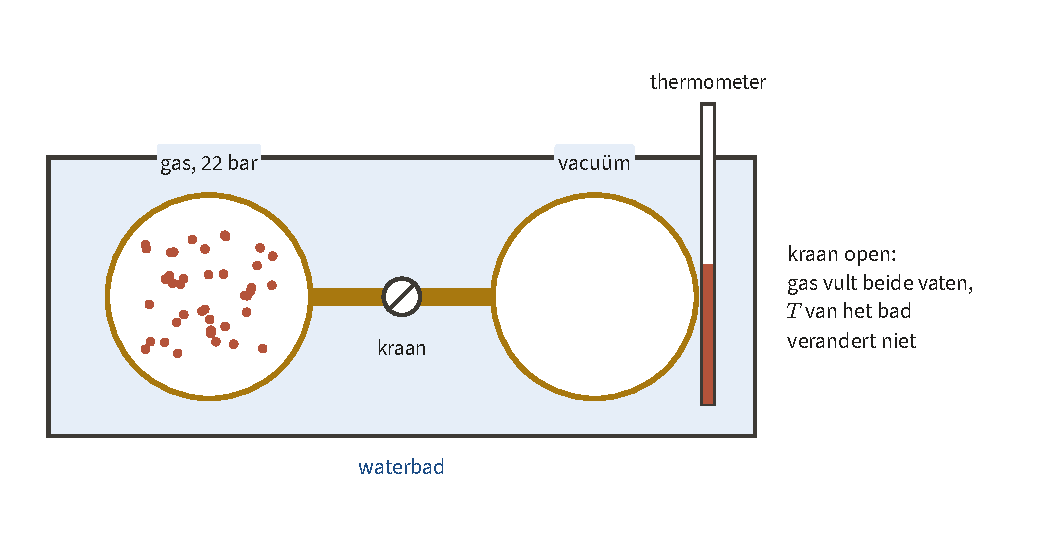
\includegraphics[width=0.8\linewidth]{Figuren/vrije_expansie}
    \caption{De vrije expansie van Joule. Na het openen van de kraan vult het gas beide vaten, terwijl de temperatuur van het bad gelijk blijft: de interne energie van het gas verandert niet, en toch verloopt het proces vanzelf in \'e\'en richting.}
    \label{fig:vrije-expansie}
\end{figure}

\paragraph{Endotherme processen die vanzelf verlopen.} Een ijsblokje in een glas limonade smelt en neemt daarbij warmte op: de enthalpie van het water stijgt. Ammoniumnitraat lost vanzelf op in water, terwijl de oplossing zo sterk afkoelt dat men er koude kompressen mee maakt. De energie van het systeem stijgt hier, en toch verloopt het proces vanzelf.

Er is dus een tweede principe nodig, naast het behoud van energie, om de richting van een proces te voorspellen. De sleutel ligt in een vaststelling die alle voorbeelden gemeen hebben: het systeem evolueert telkens naar een toestand die op moleculair niveau veel \emph{waarschijnlijker} is dan de begintoestand. Om dat te begrijpen, moeten we leren tellen.

\subsection{Microtoestanden en macrotoestanden}
\label{sec:waarschijnlijkheid-entropie}

Druk, volume, temperatuur en samenstelling beschrijven een gas als geheel. Zo'n beschrijving heet een \emph{macrotoestand}. Op moleculair niveau heeft elke molecule op elk ogenblik een eigen positie en een eigen energie. Een volledige opgave van alle posities en energie\"en heet een \emph{microtoestand}. Bij \'e\'en macrotoestand horen ontelbaar veel microtoestanden: de moleculen bewegen voortdurend en wisselen van plaats, maar de druk en temperatuur die je meet, blijven dezelfde.

Neem opnieuw het vat van Joule, maar nu met slechts vier moleculen, die we a, b, c en d noemen. Elke molecule kan zich in de linker- of de rechterhelft bevinden, onafhankelijk van de andere. Er zijn dus $2 \times 2 \times 2 \times 2 = 2^4 = 16$ microtoestanden, en omdat de moleculen voortdurend bewegen, is elk ervan even waarschijnlijk. Groeperen we ze volgens het aantal moleculen links (de macrotoestand), dan vinden we:
\begin{itemize}
\item alle vier links: 1 microtoestand (abcd);
\item drie links: 4 microtoestanden (abc, abd, acd, bcd);
\item twee links: 6 microtoestanden (ab, ac, ad, bc, bd, cd);
\item \'e\'en links: 4, en geen enkele links: 1.
\end{itemize}
De gelijkmatige verdeling is het waarschijnlijkst (6 kansen op 16), maar ``alles links'' is met 1 kans op 16 nog heel goed mogelijk (figuur~\ref{fig:microtoestanden}, links). Met duizend moleculen ligt dat helemaal anders. Het aantal microtoestanden met $n$ moleculen links is dan $1000!/(n!\,(1000-n)!)$, en de verdeling wordt een smalle piek rond de helft (figuur~\ref{fig:microtoestanden}, rechts). De kans dat alle moleculen links zitten, is $2^{-1000} \approx 10^{-301}$. Een mol gas bevat $6\times10^{23}$ moleculen: de kans op een merkbare afwijking van de gelijkmatige verdeling is daar zo klein dat je ze in de hele levensduur van het heelal nooit zou zien.

\begin{figure}[htb]
    \centering
    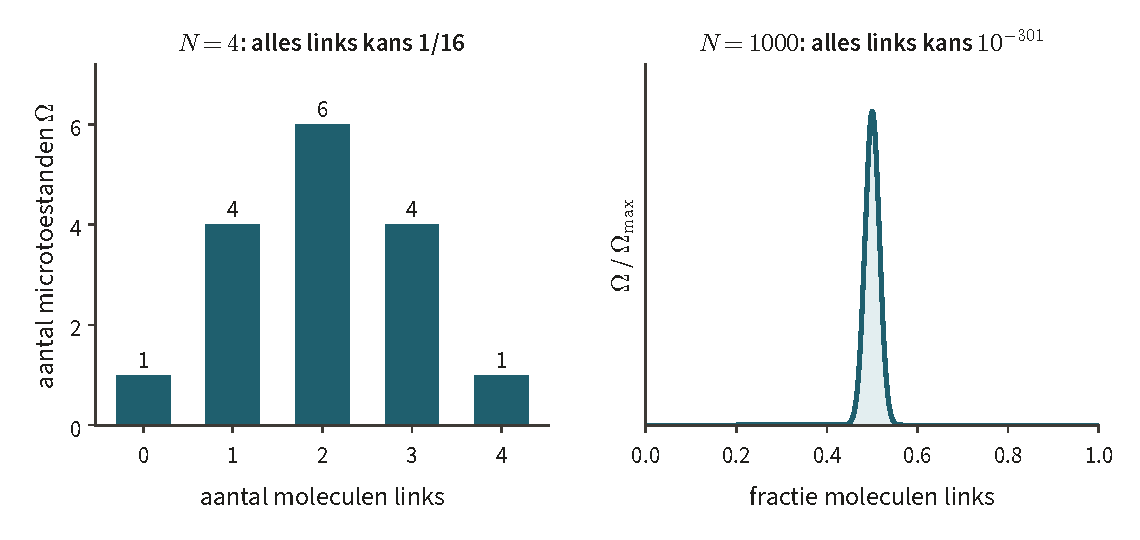
\includegraphics[width=0.9\linewidth]{Figuren/microtoestanden}
    \caption{Aantal manieren om moleculen over twee helften van een vat te verdelen. Links: bij vier moleculen is een ongelijke verdeling nog vrij waarschijnlijk. Rechts: bij duizend moleculen is de verdeling al zeer scherp rond de helft. Bij een mol gas is de kans op een merkbare afwijking praktisch nul.}
    \label{fig:microtoestanden}
\end{figure}

Dat verklaart de proef van Joule. Geen kracht duwt het gas naar het lege vat. De moleculen bewegen willekeurig, en daardoor belandt het systeem in de macrotoestand met de meeste microtoestanden, gewoon omdat die overweldigend waarschijnlijker is. De terugweg is niet verboden, maar zo onwaarschijnlijk dat hij in de praktijk nooit voorkomt.

\subsection{De formule van Boltzmann}

Ludwig Boltzmann gaf in 1877 een naam aan dit getal: hij verbond het aantal microtoestanden $\Omega$ van een macrotoestand met de \emph{entropie} $S$,
\begin{equation}
\boxed{S = k_B \ln \Omega}
\label{eq:boltzmann}
\end{equation}
met de constante van Boltzmann $k_B = R/N_A = \SI{1.381e-23}{\joule\per\kelvin}$. De formule staat op zijn grafsteen in Wenen.

\paragraph{Waarom een logaritme?} Waarom niet gewoon $S \propto \Omega$? Het antwoord volgt uit een eigenschap die we van entropie verwachten: ze moet \emph{extensief} zijn, zoals volume of massa. Voeg je twee identieke, onafhankelijke systemen samen, dan moet de entropie verdubbelen: $S_\text{tot} = S_A + S_B$. We volgen de redenering in drie stappen.
\begin{enumerate}
\item \emph{Microtoestanden vermenigvuldigen.} Voor elk van de $\Omega_A$ microtoestanden van systeem A kan systeem B zich in elk van zijn $\Omega_B$ microtoestanden bevinden. Het totale aantal combinaties is dus het \emph{product} $\Omega_\text{tot} = \Omega_A\,\Omega_B$. Zo hebben twee dobbelstenen niet $6 + 6 = 12$, maar $6 \times 6 = 36$ mogelijke uitkomsten.
\item \emph{Entropie moet optellen.} Met $S \propto \Omega$ zou het samenvoegen van twee identieke systemen de entropie niet verdubbelen maar kwadrateren. Hebben A en B elk $\Omega = 10^3$ microtoestanden, dan heeft het geheel er $10^6$: niet twee keer, maar duizend keer zoveel.
\item \emph{De logaritme zet een product om in een som.} We hebben een functie nodig met $f(\Omega_A\Omega_B) = f(\Omega_A) + f(\Omega_B)$. Dat is precies de eigenschap van de logaritme, en ze is de enige functie die eraan voldoet. In het voorbeeld: $\ln(10^6) = 6\ln 10 = 2 \times (3\ln 10) = 2\ln(10^3)$. De logaritme van het geheel is wel precies het dubbele van die van elk deel.
\end{enumerate}
De logaritme blijft bovendien stijgen met $\Omega$: een macrotoestand met meer microtoestanden heeft een hogere entropie. De constante $k_B$ is enkel een schaalfactor, zo gekozen dat de statistische entropie dezelfde waarde en eenheid (\si{\joule\per\kelvin}) heeft als de klassieke entropie die Clausius al eerder uit warmtemetingen had afgeleid (\S\ref{sec:tweedehoofdwet}).

Entropie is dus een maat voor het aantal manieren waarop een macrotoestand kan worden gerealiseerd. Mengen, warmte die van warm naar koud stroomt, een gas dat expandeert: telkens gaat het systeem naar een toestand met meer microtoestanden, dus met een hogere entropie. We maken dat nu kwantitatief voor twee situaties die je als ingenieur steeds tegenkomt: een gas dat uitzet, en twee stoffen die mengen.

\subsubsection{Entropieverandering bij isotherme expansie}

We berekenen hoeveel de entropie stijgt wanneer een ideaal gas bij constante temperatuur uitzet van $V_1$ naar $V_2$, zoals in de proef van Joule.
\begin{enumerate}
\item \emph{Tel de plaatsen voor \'e\'en molecule.} Verdeel het volume, louter als rekenhulp, in kleine cellen met volume $v_0$. Een molecule heeft dan $V/v_0$ mogelijke plaatsen (figuur~\ref{fig:expansie-cellen}).
\item \emph{Tel de schikkingen voor $N$ moleculen.} In een ideaal gas be\"invloeden de moleculen elkaar niet, dus elke molecule kiest onafhankelijk. Net als bij de dobbelstenen vermenigvuldigen de mogelijkheden: $\Omega \propto (V/v_0)^N$.
\item \emph{Neem de verhouding.} Bij constante temperatuur verandert de verdeling van de energie niet, enkel het aantal plaatsen. Dus $\Omega_2/\Omega_1 = (V_2/V_1)^N$; de willekeurige celgrootte $v_0$ valt weg.
\item \emph{Pas Boltzmann toe.} $\Delta S = k_B\ln\Omega_2 - k_B\ln\Omega_1 = k_B\ln(\Omega_2/\Omega_1) = Nk_B\ln(V_2/V_1)$. Met $N = nN_A$ en $k_BN_A = R$:
\end{enumerate}
\begin{equation}
\boxed{\Delta S = nR\ln\frac{V_2}{V_1} \qquad \text{(isotherme expansie van een ideaal gas)}}
\label{eq:dS-expansie}
\end{equation}

\begin{figure}[htb]
    \centering
    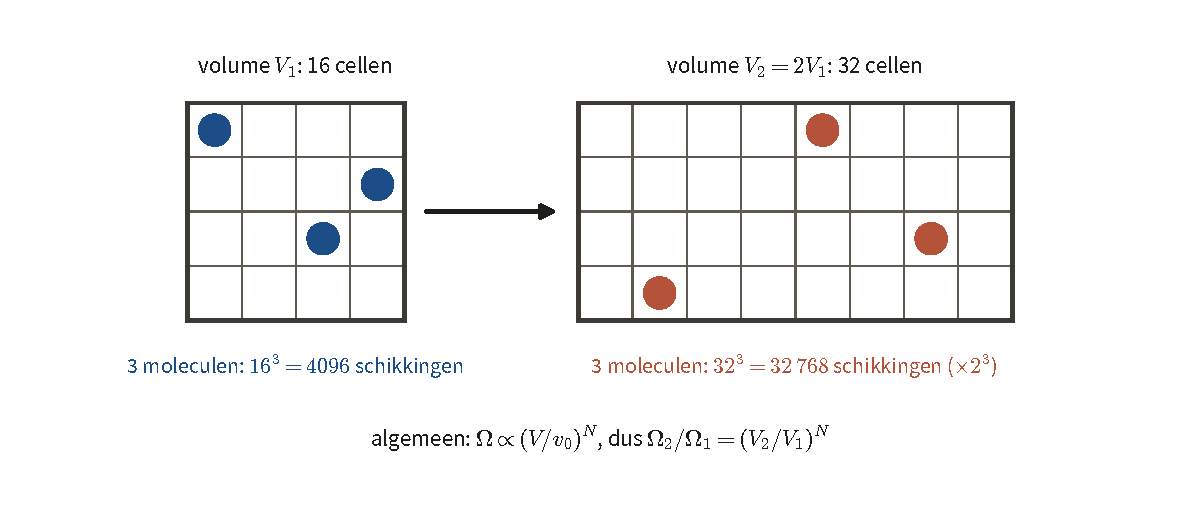
\includegraphics[width=0.85\linewidth]{Figuren/expansie_cellen}
    \caption{Verdubbelt het volume, dan verdubbelt het aantal plaatsen voor elke molecule. Voor drie moleculen stijgt het aantal schikkingen met een factor $2^3 = 8$, voor $N$ moleculen met $2^N$.}
    \label{fig:expansie-cellen}
\end{figure}

\begin{voorbeeld}{Entropie bij een volumeverdubbeling}
\SI{1}{\mole} ideaal gas zet bij constante temperatuur uit van \SI{10}{\litre} naar \SI{20}{\litre}:
\[
\Delta S = nR\ln\frac{V_2}{V_1} = (1)(8.314)\ln 2 = \SI{5.76}{\joule\per\kelvin}.
\]
Een klein getal, maar achter die \SI{5.76}{\joule\per\kelvin} zit een gigantische toename van het aantal microtoestanden: $\Omega_2/\Omega_1 = 2^{6\times10^{23}}$. De logaritme maakt er een hanteerbaar getal van.
\end{voorbeeld}

Merk op dat in deze afleiding nergens warmte of arbeid voorkomt: het resultaat volgt enkel uit tellen. In \S\ref{sec:tweedehoofdwet} zullen we dezelfde formule terugvinden langs een heel andere weg, uit een warmtemeting.

\subsubsection{Entropieverandering bij mengen}

Bij mengen gaat het niet om meer plaatsen, maar om meer manieren om twee soorten moleculen over dezelfde plaatsen te verdelen. Verdeel $N_A$ moleculen A en $N_B$ moleculen B over $N = N_A + N_B$ plaatsen van een rooster.
\begin{enumerate}
\item \emph{Tel de schikkingen.} Zolang A en B gescheiden zijn, elk in hun eigen deel, is er voor het patroon maar \'e\'en schikking: $\Omega = 1$. Na het mengen kies je welke $N_A$ van de $N$ plaatsen door A worden ingenomen; de rest is voor B. Dat kan op
\[
\Omega = \frac{N!}{N_A!\,N_B!}
\]
manieren. Voor een klein rooster met 8 moleculen A en 8 moleculen B is dat al $16!/(8!\,8!) = 12\,870$ (figuur~\ref{fig:menging-rooster}).
\item \emph{Vereenvoudig met Stirling.} Voor grote getallen geldt $\ln x! \approx x\ln x - x$ (de benadering van Stirling, al op een procent nauwkeurig vanaf $x = 100$). Zo wordt
\[
\ln\Omega \approx N\ln N - N_A\ln N_A - N_B\ln N_B ,
\]
waarbij de termen $-N + N_A + N_B$ wegvallen.
\item \emph{Schrijf in molfracties.} Splits $N\ln N = N_A\ln N + N_B\ln N$ en groepeer: $\ln\Omega = -N_A\ln(N_A/N) - N_B\ln(N_B/N) = -N_A\ln x_A - N_B\ln x_B$.
\item \emph{Pas Boltzmann toe en reken per mol.} Met $\Delta S = k_B\ln\Omega$, $N_i = n_iN_A$ en $k_BN_A = R$ volgt, gedeeld door het totale aantal mol:
\end{enumerate}
\begin{equation}
\boxed{\Delta S_{\text{meng}} = -R\bigl(x_A\ln x_A + x_B\ln x_B\bigr) > 0 .}
\label{eq:mengentropie}
\end{equation}
Omdat elke molfractie kleiner is dan 1, is elke $\ln x_i$ negatief, en is de mengentropie altijd positief: mengen verhoogt altijd het aantal microtoestanden. Ze is maximaal bij een 50/50-mengsel.

\begin{figure}[htb]
    \centering
    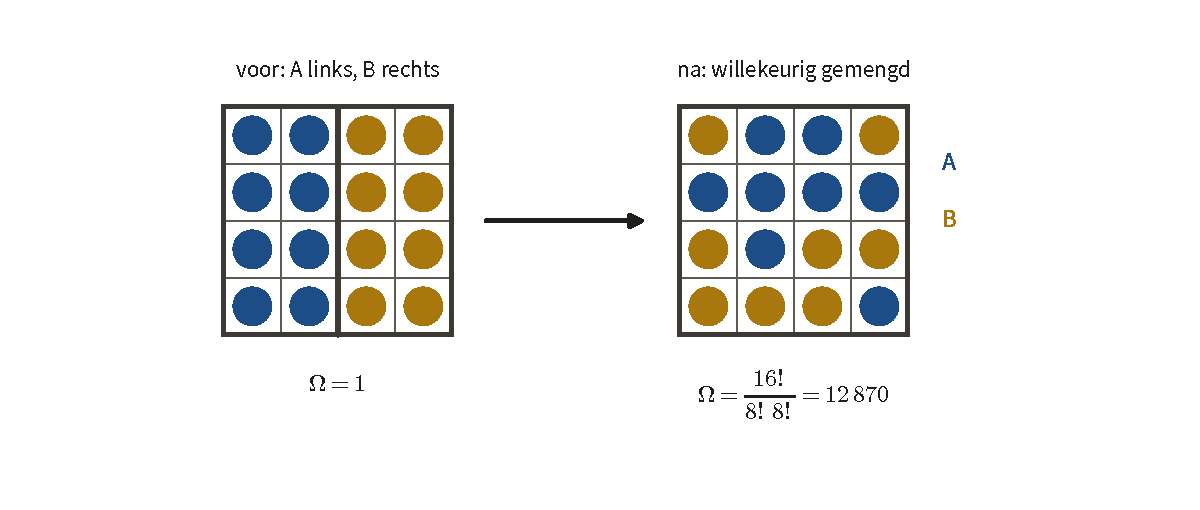
\includegraphics[width=0.85\linewidth]{Figuren/menging_rooster}
    \caption{Mengen op een rooster. Gescheiden is er \'e\'en schikking van A en B; gemengd zijn er voor dit kleine rooster al 12\,870. Bij een mol moleculen loopt dat op tot een getal met $10^{23}$ cijfers.}
    \label{fig:menging-rooster}
\end{figure}

\begin{voorbeeld}{Mengentropie van lucht, en de minimale arbeid om ze te scheiden}
Voor een 50/50-mengsel van \ce{N2} en \ce{O2} is $\Delta S_\text{meng} = -R(0.5\ln 0.5 + 0.5\ln 0.5) = R\ln 2 = \SI{5.76}{\joule\per\mole\per\kelvin}$: precies dezelfde waarde als bij de volumeverdubbeling. Dat is geen toeval: na het mengen heeft elke molecule twee keer zoveel ruimte, net als bij de expansie.

Echte lucht bevat \SI{79}{\percent} \ce{N2} en \SI{21}{\percent} \ce{O2} (argon rekenen we bij de stikstof):
\[
\Delta S_\text{meng} = -R(0.79\ln 0.79 + 0.21\ln 0.21) = (8.314)(0.186 + 0.328) = \SI{4.27}{\joule\per\mole\per\kelvin}.
\]
Omgekeerd verloopt het scheiden van lucht nooit vanzelf: het kost arbeid. Hoeveel minstens, zie je in oefening~\ref{oef:meng-scheiden}: het komt neer op $T\Delta S_\text{meng} \approx (298)(4.27) = \SI{1.3}{\kilo\joule}$ per mol lucht. Een echte luchtscheidingsinstallatie, die de stikstof voor de ammoniakfabriek levert, verbruikt vijf tot tien keer meer. Waar die extra arbeid verloren gaat, is een vraag voor de scheidingstechnologie.
\end{voorbeeld}

\begin{figure}[htb]
    \centering
    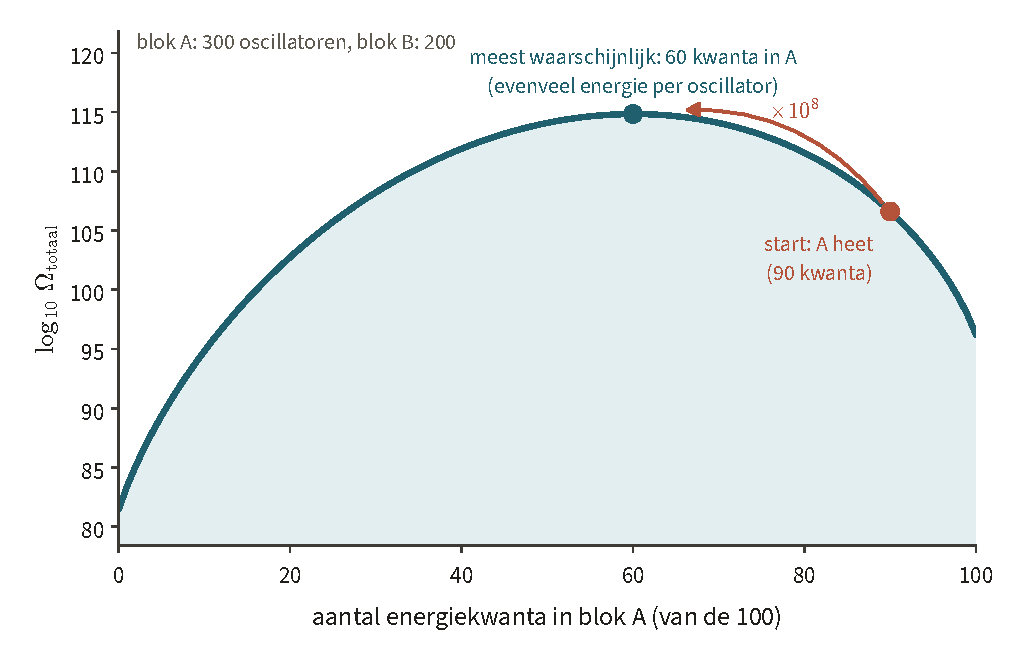
\includegraphics[width=0.75\linewidth]{Figuren/twee_blokken}
    \caption{Twee blokken in thermisch contact delen 100 energiekwanta. Blok A heeft 300 trillende atomen (oscillatoren), blok B 200. Voor elke verdeling is $\Omega_\text{totaal} = \Omega_A\Omega_B$ uitgezet (logaritmische schaal). Start A met 90 kwanta (heet), dan zijn er $10^8$ keer meer microtoestanden wanneer de energie zich herverdeelt tot evenveel energie per oscillator.}
    \label{fig:twee-blokken}
\end{figure}

\begin{casusuitgewerkt}{waarom stroomt warmte enkel van warm naar koud?}
Bekijk twee kleine blokken die energiekwanta uitwisselen (figuur~\ref{fig:twee-blokken}). Een blok met $N$ trillende atomen en $q$ kwanta kan die kwanta op
\[
\Omega(N,q) = \frac{(q+N-1)!}{q!\,(N-1)!}
\]
manieren verdelen (het aantal manieren om $q$ gelijke ballen over $N$ dozen te verdelen). Samen is $\Omega_\text{totaal} = \Omega_A\Omega_B$.

\emph{Stap 1: de begintoestand.} Blok A (300 atomen) heeft 90 van de 100 kwanta, blok B (200 atomen) slechts 10. Per atoom heeft A dus zes keer meer energie: A is heet, B is koud. Er zijn $10^{106.6}$ microtoestanden.

\emph{Stap 2: de evenwichtstoestand.} Het maximum ligt bij 60 kwanta in A en 40 in B: evenveel energie per atoom, dus dezelfde temperatuur. Daar zijn er $10^{114.8}$ microtoestanden, $10^8$ keer meer.

\emph{Stap 3: het besluit.} Botsingen verdelen de kwanta voortdurend opnieuw, zonder voorkeur. Het systeem belandt daardoor bijna zeker in de verdeling met de meeste microtoestanden. Warmte stroomt van warm naar koud, niet omdat een kracht haar duwt, maar omdat er overweldigend veel meer manieren zijn om de energie gelijkmatig te verdelen. Met 100 kwanta is de terugweg naar 90 kwanta in A al honderd miljoen keer minder waarschijnlijk; voor een kop koffie met $10^{25}$ moleculen is hij onmogelijk. Hetzelfde geldt voor de buitenlucht en de woning: de warmte gaat vanzelf naar buiten, nooit naar binnen.

\emph{Volgende vraag.} Een warmtepomp dwingt de warmte toch de ``verkeerde'' kant op. Hoe reken je uit hoeveel arbeid dat minstens kost, zonder microtoestanden te tellen?
\end{casusuitgewerkt}

\section{De tweede hoofdwet en de klassieke formulering van entropie}
\label{sec:tweedehoofdwet}

\begin{casus}{hoeveel stroom vraagt een warmtepomp?}
Een warmtepomp levert \SI{10}{\kilo\watt} warmte aan een vloerverwarming van \SI{35}{\celsius}, terwijl het buiten \SI{5}{\celsius} is. Hoeveel elektrisch vermogen heeft de compressor daar minstens voor nodig? En hoeveel als de woning radiatoren van \SI{55}{\celsius} heeft?

\emph{Schat eerst zelf:} moet de compressor evenveel arbeid leveren als de warmte die binnenkomt, meer, of veel minder? Waarom zou de afgiftetemperatuur ertoe doen?
\end{casus}


\subsection{De tweede hoofdwet van de thermodynamica}

De tweede hoofdwet werd niet ontdekt door moleculen te tellen, maar door naar stoommachines te kijken. Sadi Carnot vroeg zich in 1824 af hoeveel arbeid een stoommachine maximaal uit een hoeveelheid steenkool kan halen. Hij en later Kelvin en Clausius stelden vast dat elke warmtemachine een deel van de opgenomen warmte moet afgeven aan een koudere omgeving, hoe goed ze ook gebouwd is. Uit die ervaring formuleerden ze twee gelijkwaardige uitspraken:
\begin{itemize}
\item \emph{Kelvin (1851):} geen enkele machine die een kringloop doorloopt, kan warmte uit \'e\'en reservoir volledig omzetten in arbeid.
\item \emph{Clausius (1850):} warmte stroomt nooit vanzelf van een koud naar een warm lichaam.
\end{itemize}
Beide uitspraken zijn veralgemeningen van ontelbare waarnemingen; niemand heeft ooit een tegenvoorbeeld gevonden. Boltzmann toonde later waarom: ze zijn het macroscopische gevolg van het tellen van microtoestanden. Een ge\"isoleerd systeem gaat naar de macrotoestand met de meeste microtoestanden, dus met de hoogste entropie. Dat geeft de algemeenste vorm van de wet.

\begin{definitie}{Tweede hoofdwet van de thermodynamica}
De totale entropie van een ge\"isoleerd systeem neemt bij elk spontaan proces toe:
\begin{equation}
\Delta S_{\text{univ}} \geq 0,
\end{equation}
met het gelijkheidsteken enkel voor een reversibel proces.
\end{definitie}

Het woord ``universum'' klinkt groots, maar betekent hier gewoon: het systeem samen met alles waarmee het energie uitwisselt, zodat het geheel ge\"isoleerd is. Voor een kop koffie op tafel is dat de koffie plus de kamer. De eerste hoofdwet gaat over de \emph{hoeveelheid} energie, de tweede over de \emph{richting} waarin processen lopen.

\subsection{De Clausius-definitie: entropie uit warmte}

Microtoestanden tellen lukt voor een ideaal gas of een eenvoudig model, maar niet voor de stoom in een turbine of het koelmiddel in een warmtepomp. Voor de ingenieur is een tweede, gelijkwaardige definitie veel bruikbaarder. Clausius vond al in 1865, nog v\'o\'or Boltzmann, dat je de entropieverandering kan \emph{meten} via de warmte die een systeem reversibel opneemt:
\begin{equation}
\boxed{\dd S = \frac{\delta Q_{\text{rev}}}{T}}
\label{eq:clausius}
\end{equation}

\paragraph{Waarom warmte gedeeld door temperatuur?} Twee vaststellingen maken die vorm aannemelijk.
\begin{enumerate}
\item \emph{Warmte verhoogt het aantal microtoestanden.} Voeg je energie toe aan een systeem, dan zijn er meer kwanta om over de moleculen te verdelen, en dus meer manieren om dat te doen. Arbeid die reversibel een zuiger verplaatst, doet dat niet: ze verandert enkel het volume of de positie, op een ordelijke manier. Daarom staat in de teller warmte, geen arbeid.
\item \emph{Dezelfde warmte doet meer bij lage temperatuur.} Een koud systeem heeft weinig energie, verdeeld over weinig kwanta. Wat extra energie zet daar relatief veel nieuwe verdelingen open. Een warm systeem bevat al veel energie; dezelfde portie verandert er relatief weinig. Vergelijk het met niezen: in een stille bibliotheek valt het op, op een drukke markt niemand. Daarom staat $T$ in de noemer.
\end{enumerate}

\paragraph{Toets 1: warmte van warm naar koud.} Laat \SI{1000}{\joule} warmte stromen van koffie van \SI{80}{\celsius} naar een kamer van \SI{20}{\celsius} (figuur~\ref{fig:warmtestroom-entropie}). Beide zijn zo groot dat hun temperatuur nauwelijks verandert. De koffie verliest $1000/353 = \SI{2.83}{\joule\per\kelvin}$ entropie, de kamer wint $1000/293 = \SI{3.41}{\joule\per\kelvin}$. Samen is $\Delta S_\text{univ} = \SI{+0.58}{\joule\per\kelvin}$: het proces verloopt vanzelf. De omgekeerde richting zou $\SI{-0.58}{\joule\per\kelvin}$ geven, en is dus onmogelijk. De definitie van Clausius levert zo precies de uitspraak van Clausius op, en de tweeblokkenproef van de casus in getallen.

\begin{figure}[htb]
    \centering
    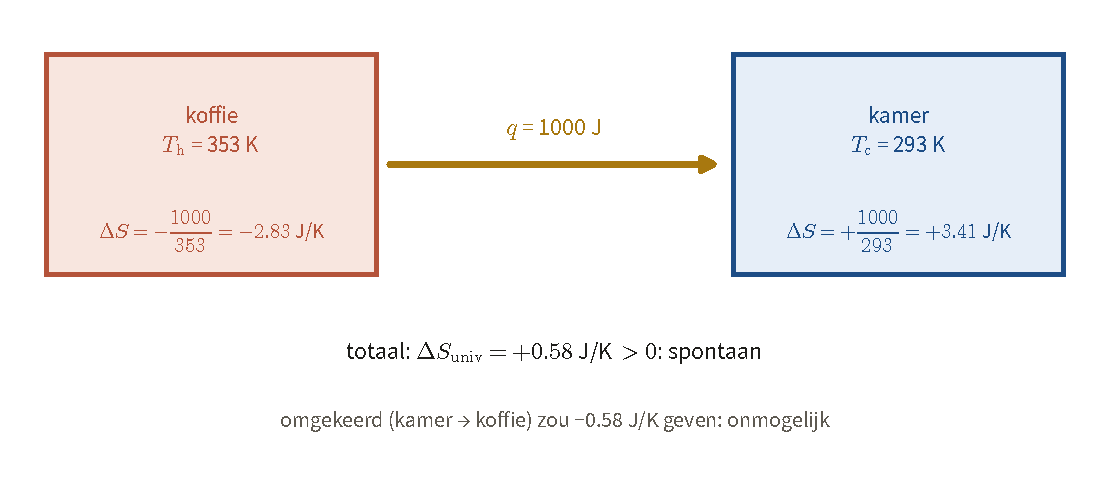
\includegraphics[width=0.8\linewidth]{Figuren/warmtestroom_entropie}
    \caption{Entropiebalans voor \SI{1}{\kilo\joule} warmte die van hete koffie naar de kamer stroomt. Dezelfde warmte verhoogt de entropie van de koude kamer meer dan ze die van de warme koffie verlaagt.}
    \label{fig:warmtestroom-entropie}
\end{figure}

\paragraph{Toets 2: dezelfde formule als Boltzmann.} Laat \SI{1}{\mole} ideaal gas reversibel en isotherm uitzetten van $V_1$ naar $V_2$, door een zuiger heel langzaam te laten wijken terwijl het gas in contact staat met een warmtebad. In hoofdstuk~\ref{ch:energie} zagen we twee dingen: bij constante temperatuur is $\Delta U = 0$ voor een ideaal gas, en de arbeid is $W = -nRT\ln(V_2/V_1)$. Uit de eerste hoofdwet volgt $Q_\text{rev} = -W = nRT\ln(V_2/V_1)$, en met Clausius
\[
\Delta S = \frac{Q_\text{rev}}{T} = nR\ln\frac{V_2}{V_1}.
\]
Dat is exact vergelijking~\eqref{eq:dS-expansie}, die we uit het tellen van cellen haalden. Twee volledig verschillende redeneringen, de ene met warmte en temperatuur, de andere met microtoestanden, leveren dezelfde entropie. Dat is de sterkste aanwijzing dat beide over dezelfde grootheid gaan.

\paragraph{Toets 3: een irreversibel proces.} Nu de vrije expansie van Joule, tussen dezelfde begin- en eindtoestand. Het gas neemt geen warmte op ($Q = 0$). Toch is de entropie gestegen met $nR\ln(V_2/V_1)$, want entropie is een toestandsfunctie: ze hangt enkel af van begin- en eindtoestand, en die zijn dezelfde als bij de reversibele expansie. Bij een irreversibel proces is de entropietoename dus \emph{groter} dan $Q/T$. Dat geeft de \emph{ongelijkheid van Clausius}:
\begin{equation}
\dd S \geq \frac{\delta Q}{T},
\end{equation}
met het gelijkheidsteken enkel voor een reversibel proces. Het verschil is de entropie die door het proces zelf wordt \emph{geproduceerd}: door wrijving, door warmte die over een eindig temperatuurverschil stroomt, door menging, of zoals hier door een gas dat ongeremd uitzet.

Uit toets 3 volgt ook de praktische werkwijze om een entropieverandering te berekenen: omdat $S$ een toestandsfunctie is, kies je altijd een \emph{denkbeeldige reversibele weg} tussen dezelfde begin- en eindtoestand, ook als het echte proces irreversibel was, en berekent daarlangs $\int\delta Q_\text{rev}/T$. Twee zulke wegen komen in de praktijk telkens terug: een faseovergang en het opwarmen van een stof.

\subsubsection{Entropie bij faseovergangen}
\label{sec:entropie-faseovergangen}

In hoofdstuk~\ref{ch:energie} (figuur~\ref{fig:opwarmcurve}) zagen we dat de temperatuur tijdens het smelten of koken constant blijft: alle toegevoerde warmte gaat naar het verbreken van intermoleculaire bindingen, niet naar snellere beweging. Bij constante druk is die warmte de faseovergangsenthalpie, en ze wordt bij \'e\'en vaste temperatuur opgenomen. In vergelijking~\eqref{eq:clausius} is $T$ dan constant, en de integratie is onmiddellijk:
\begin{equation}
\Delta S_{\text{trans}} = \frac{\Delta H_{\text{trans}}}{T_{\text{trans}}} .
\label{eq:entropie_fase}
\end{equation}
Voor water vind je
\[
\Delta S_\text{fus} = \frac{6010}{273.15} = \SI{22.0}{\joule\per\mole\per\kelvin},
\qquad
\Delta S_\text{vap} = \frac{40\,700}{373.15} = \SI{109}{\joule\per\mole\per\kelvin}.
\]
De verdampingsentropie is vijf keer groter dan de smeltentropie. Moleculair is dat logisch: bij smelten blijven de moleculen dicht op elkaar, ze krijgen enkel vrijheid om langs elkaar te bewegen en te draaien. Bij verdampen neemt elke molecule ongeveer 1700 keer meer volume in, en met $nR\ln(V_2/V_1)$ is dat alleen al $R\ln 1700 = \SI{62}{\joule\per\mole\per\kelvin}$. Vergelijking~\eqref{eq:entropie_fase} is ook de basis van de vergelijking van Clapeyron (hoofdstuk~\ref{ch:niet-reagerend}).

\subsubsection{Entropieverandering bij opwarming}
\label{sec:entropie-opwarming}

Warm je een stof op zonder dat ze van fase verandert, dan stijgt de temperatuur tijdens het opnemen van de warmte. We leiden de entropieverandering af in drie stappen.
\begin{enumerate}
\item \emph{Een klein stapje.} Bij constante druk is de warmte om de temperatuur met $\dd T$ te verhogen $\delta Q_\text{rev} = nC_p\,\dd T$ (hoofdstuk~\ref{ch:energie}). Langzaam opwarmen, telkens met een bad dat net iets warmer is, maakt dat reversibel.
\item \emph{Deel door $T$.} Volgens Clausius is $\dd S = nC_p\,\dd T/T$.
\item \emph{Tel alle stapjes op.} Integreer van $T_1$ tot $T_2$. Voor constante $C_p$:
\end{enumerate}
\begin{equation}
\boxed{\Delta S = \int_{T_1}^{T_2}\frac{nC_p}{T}\,\dd T = nC_p\ln\frac{T_2}{T_1}}
\qquad\text{(constante $C_p$)}.
\label{eq:dS-opwarming}
\end{equation}
Waar de enthalpie lineair stijgt met de temperatuur, $\Delta H = nC_p\,\Delta T$, stijgt de entropie logaritmisch: elke volgende joule wordt bij een hogere temperatuur toegevoegd en levert dus minder entropie op. Bij constant volume geldt dezelfde formule met $C_V$. Over een traject met faseovergangen tel je de stukken gewoon op: opwarmen met vergelijking~\eqref{eq:dS-opwarming}, faseovergangen met vergelijking~\eqref{eq:entropie_fase} (figuur~\ref{fig:entropie-opwarming}).

\begin{figure}[htb]
    \centering
    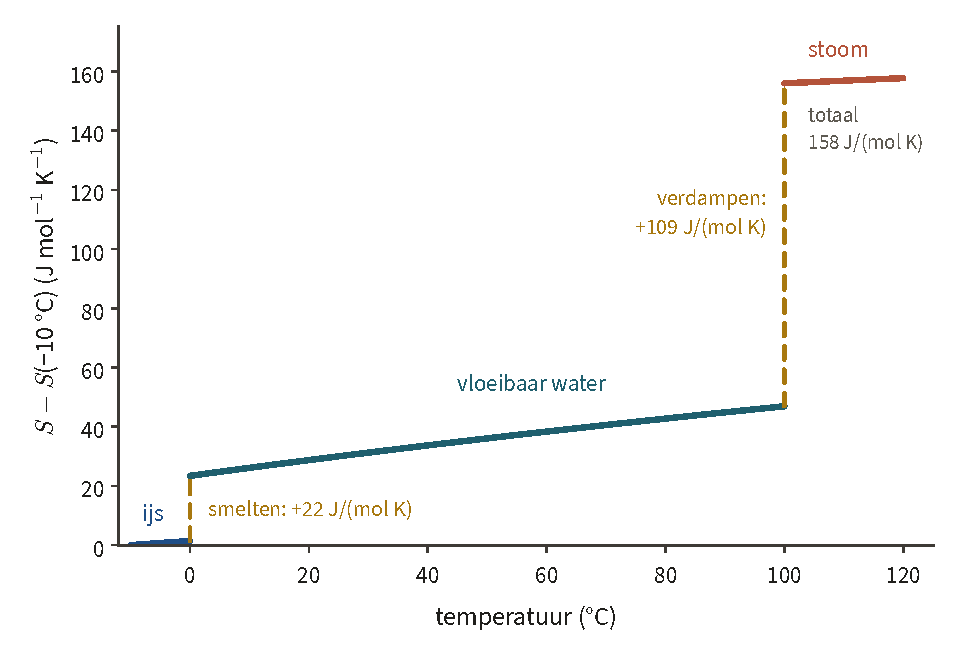
\includegraphics[width=0.75\linewidth]{Figuren/entropie_opwarming_water}
    \caption{Entropie van \SI{1}{\mole} water bij \SI{1}{\bar}, van ijs bij \SI{-10}{\celsius} tot stoom bij \SI{120}{\celsius}. Elke opwarmfase volgt vergelijking~\eqref{eq:dS-opwarming}; bij smelten en verdampen springt de entropie verticaal omhoog. De sprong bij verdampen is vijf keer groter dan die bij smelten: een gas heeft veel meer microtoestanden dan een vloeistof.}
    \label{fig:entropie-opwarming}
\end{figure}

\begin{voorbeeld}{Van ijs bij $-10\,^\circ$C tot stoom bij $120\,^\circ$C}
We berekenen de entropieverandering wanneer \SI{1}{\mole} water bij \SI{1}{\bar} wordt opgewarmd van ijs bij \SI{263.15}{\kelvin} tot stoom bij \SI{393.15}{\kelvin}. Gegevens: $C_p$ = 38.0 (ijs), 75.3 (water) en 33.6 (stoom) \si{\joule\per\mole\per\kelvin}; $\Delta H_\text{fus} = \SI{6.01}{\kilo\joule\per\mole}$ bij \SI{273.15}{\kelvin}; $\Delta H_\text{vap} = \SI{40.7}{\kilo\joule\per\mole}$ bij \SI{373.15}{\kelvin}. Het traject bestaat uit vijf stappen.

\textbf{1. IJs opwarmen} van 263.15 naar \SI{273.15}{\kelvin}: $\Delta S_1 = 38.0\ln(273.15/263.15) = (38.0)(0.0373) = \SI{1.42}{\joule\per\mole\per\kelvin}$.

\textbf{2. Smelten} bij \SI{273.15}{\kelvin}: $\Delta S_2 = 6010/273.15 = \SI{22.00}{\joule\per\mole\per\kelvin}$.

\textbf{3. Water opwarmen} van 273.15 naar \SI{373.15}{\kelvin}: $\Delta S_3 = 75.3\ln(373.15/273.15) = (75.3)(0.3120) = \SI{23.49}{\joule\per\mole\per\kelvin}$.

\textbf{4. Verdampen} bij \SI{373.15}{\kelvin}: $\Delta S_4 = 40\,700/373.15 = \SI{109.07}{\joule\per\mole\per\kelvin}$.

\textbf{5. Stoom opwarmen} van 373.15 naar \SI{393.15}{\kelvin}: $\Delta S_5 = 33.6\ln(393.15/373.15) = (33.6)(0.0522) = \SI{1.75}{\joule\per\mole\per\kelvin}$.

\textbf{Totaal:} $\Delta S = 1.42 + 22.00 + 23.49 + 109.07 + 1.75 = \SI{157.7}{\joule\per\mole\per\kelvin}$.

Verdampen alleen levert bijna 70\,\% van het totaal. Het opwarmen van vloeibaar water over \SI{100}{\kelvin} kost veel meer warmte (\SI{7.5}{\kilo\joule}) dan het smelten (\SI{6.0}{\kilo\joule}), maar levert ongeveer evenveel entropie, omdat die warmte bij hogere temperatuur wordt opgenomen.
\end{voorbeeld}

\subsection{Lokale entropieafname}

De tweede hoofdwet gaat over het \emph{totaal}. De entropie van het systeem zelf mag best dalen, als de omgeving meer wint. Water dat bevriest, een eiwit dat zich opvouwt, een koelkast die haar binnenkant afkoelt: telkens wordt het systeem geordender. Om na te gaan of zo'n proces toch vanzelf kan verlopen, moet je ook de omgeving meerekenen. Dat gaat in drie stappen.
\begin{enumerate}
\item \emph{Het systeem.} De entropieverandering van het systeem bereken je zoals hierboven, of voor een reactie met getabelleerde standaardentropie\"en (\S\ref{sec:derde-hoofdwet}).
\item \emph{De omgeving.} De omgeving is groot (de lucht, het koelwater, het labo) en blijft op een vaste temperatuur $T$. Voor zo'n reservoir is elke warmte-uitwisseling reversibel, dus is haar entropieverandering gewoon de ontvangen warmte gedeeld door $T$. Bij constante druk geeft het systeem $-\Delta H$ aan warmte af, dus
\[
\Delta S_\text{omg} = -\frac{\Delta H}{T}.
\]
Een exotherme reactie ($\Delta H < 0$) verhoogt de entropie van de omgeving.
\item \emph{De som.} Het proces verloopt vanzelf als $\Delta S_\text{univ} = \Delta S + \Delta S_\text{omg} > 0$.
\end{enumerate}

\begin{voorbeeld}{De vorming van water}
Waterstof en zuurstof reageren explosief tot water: \ce{2 H2(g) + O2(g) -> 2 H2O(l)} bij \SI{298}{\kelvin} en \SI{1}{\bar}. Gegevens: $S_m^\circ$ = 130.7 (\ce{H2}), 205.2 (\ce{O2}) en 70.0 (\ce{H2O(l)}) \si{\joule\per\mole\per\kelvin}; $\Delta_fH^\circ(\ce{H2O(l)}) = \SI{-285.8}{\kilo\joule\per\mole}$.

\textbf{1. Het systeem.} 
\[
\Delta_r S^\circ = 2(70.0) - [2(130.7) + 205.2] = \SI{-326.6}{\joule\per\kelvin}.
\]
Sterk negatief: drie mol gas, met veel bewegingsvrijheid, worden twee mol vloeistof. Op basis van het systeem alleen zou je besluiten dat de reactie niet vanzelf kan verlopen, terwijl ze een van de heftigste reacties is die we kennen.

\textbf{2. De omgeving.} De reactie is sterk exotherm, $\Delta_r H^\circ = 2(-285.8) = \SI{-571.6}{\kilo\joule}$. Die warmte komt in de omgeving terecht:
\[
\Delta S_\text{omg} = -\frac{\Delta_r H^\circ}{T} = \frac{571\,600}{298} = \SI{+1917}{\joule\per\kelvin}.
\]

\textbf{3. De som.} $\Delta S_\text{univ} = -326.6 + 1917 = \SI{+1590}{\joule\per\kelvin} > 0$ (figuur~\ref{fig:entropiebalans-water}). De orde die in het systeem ontstaat, wordt ruimschoots betaald door de warmte die de omgeving opwarmt. Bij een exotherme reactie wint de omgeving bijna altijd, zeker bij lage temperatuur, waar $-\Delta H/T$ groot is.
\end{voorbeeld}

\begin{figure}[htb]
    \centering
    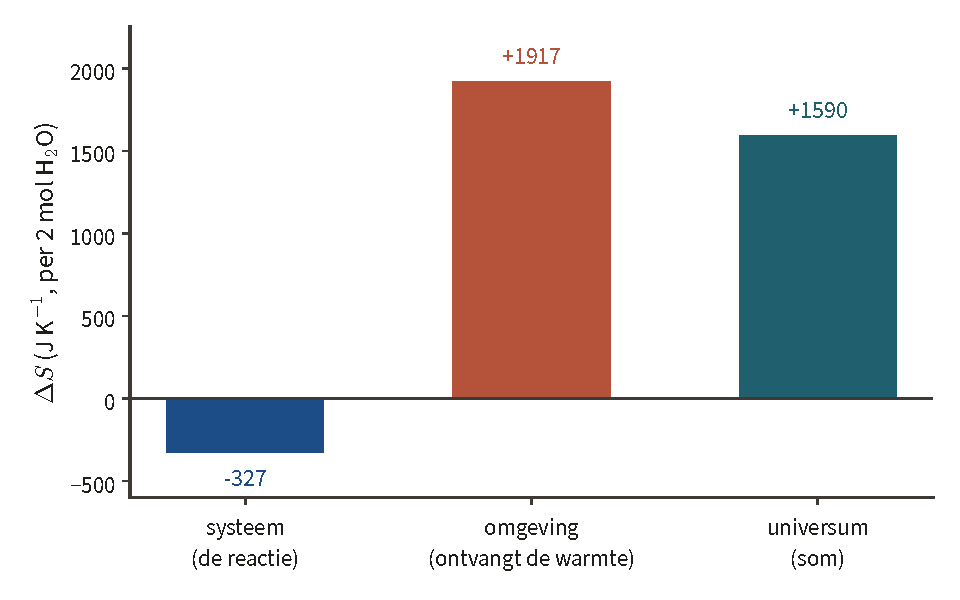
\includegraphics[width=0.65\linewidth]{Figuren/entropiebalans_water}
    \caption{Entropiebalans voor de vorming van 2 mol vloeibaar water bij \SI{298}{\kelvin}. De entropie van het systeem daalt, maar die van de omgeving stijgt bijna zes keer meer door de vrijgekomen warmte.}
    \label{fig:entropiebalans-water}
\end{figure}

Hetzelfde principe verklaart een koelkast of warmtepomp: ze maakt een ruimte kouder (lagere entropie), maar verbruikt daarvoor arbeid en dumpt meer warmte, met meer entropie, in de keuken. Hoeveel arbeid minstens nodig is, volgt uit precies zo'n balans.

\subsection{Warmtemachines, koelmachines en warmtepompen}
\label{sec:carnot}

Met de entropie kunnen we nu de grens berekenen voor elk toestel dat warmte en arbeid omzet. Bekijk een warmtepomp die in stationaire werking per cyclus warmte $Q_\mathrm{c}$ opneemt bij de lage temperatuur $T_\mathrm{c}$, arbeid $W$ ontvangt en warmte $Q_\mathrm{h} = Q_\mathrm{c} + W$ afgeeft bij de hoge temperatuur $T_\mathrm{h}$ (figuur~\ref{fig:warmtepomp}). Het koelmiddel doorloopt een kringloop en keert telkens terug naar dezelfde toestand: zijn entropie verandert over een cyclus niet. Enkel de twee warmtereservoirs veranderen van entropie: de buitenlucht verliest $Q_\mathrm{c}/T_\mathrm{c}$, de woning wint $Q_\mathrm{h}/T_\mathrm{h}$. De tweede hoofdwet eist
\[
\Delta S_\text{univ} = \frac{Q_\mathrm{h}}{T_\mathrm{h}} - \frac{Q_\mathrm{c}}{T_\mathrm{c}} \geq 0
\quad\Longrightarrow\quad
\frac{Q_\mathrm{c}}{Q_\mathrm{h}} \leq \frac{T_\mathrm{c}}{T_\mathrm{h}}.
\]
De woning moet dus minstens zoveel entropie ontvangen als de buitenlucht verliest. Omdat $T_\mathrm{h} > T_\mathrm{c}$, kan dat enkel als $Q_\mathrm{h}$ groter is dan $Q_\mathrm{c}$: het verschil is de arbeid. Met $W = Q_\mathrm{h} - Q_\mathrm{c}$ volgt voor de \emph{prestatiecoëfficiënt} (COP, \emph{coefficient of performance}):
\begin{equation}
\boxed{\;\mathrm{COP}_\text{warmtepomp} = \frac{Q_\mathrm{h}}{W} \leq \frac{T_\mathrm{h}}{T_\mathrm{h} - T_\mathrm{c}}\;}
\label{eq:cop-warmtepomp}
\end{equation}
Het gelijkheidsteken geldt voor een reversibele kringloop, de \emph{Carnot-kringloop}. Op dezelfde manier vind je de grenzen voor de twee andere toestellen:
\begin{equation}
\mathrm{COP}_\text{koelmachine} = \frac{Q_\mathrm{c}}{W} \leq \frac{T_\mathrm{c}}{T_\mathrm{h} - T_\mathrm{c}},
\qquad
\eta_\text{warmtemachine} = \frac{W}{Q_\mathrm{h}} \leq 1 - \frac{T_\mathrm{c}}{T_\mathrm{h}}.
\label{eq:carnot}
\end{equation}
Een koelmachine is dezelfde kringloop, maar het nuttige effect is de warmte die aan de koude kant wordt weggehaald. Een warmtemachine (stoomturbine, automotor) loopt de kringloop in omgekeerde zin: ze neemt warmte op bij hoge temperatuur en levert arbeid, maar moet altijd een deel van de warmte, met haar entropie, kwijt aan de koude omgeving. Alle drie de grenzen hangen enkel af van de temperaturen, niet van het koelmiddel of de constructie. Hoe kleiner het temperatuurverschil dat een warmtepomp moet overbruggen, hoe minder arbeid ze nodig heeft (figuur~\ref{fig:cop}).

\begin{figure}[htb]
    \centering
    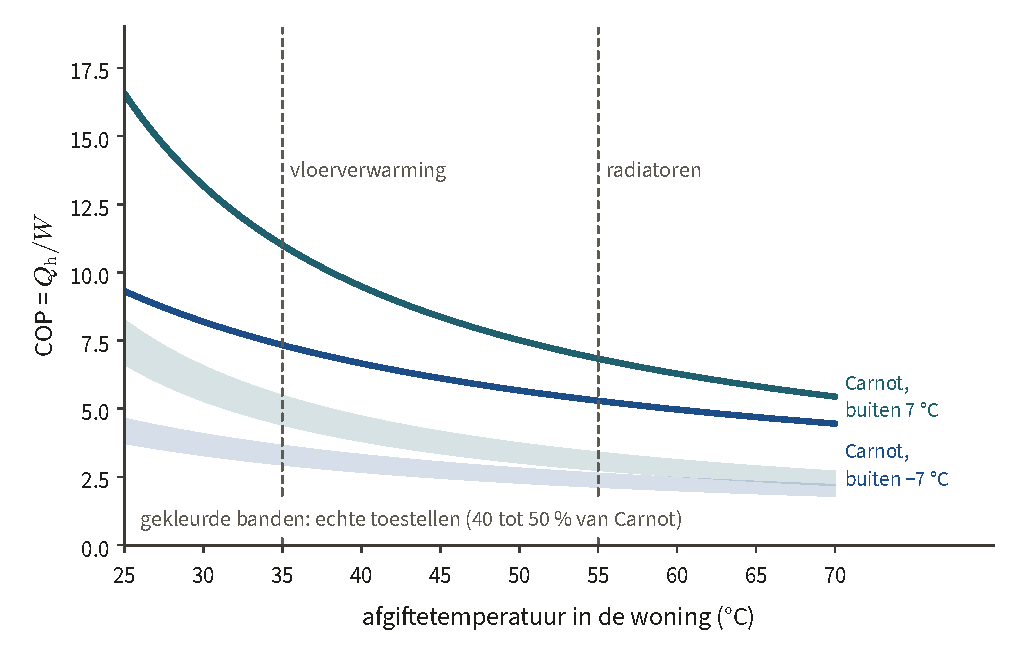
\includegraphics[width=0.75\linewidth]{Figuren/cop_warmtepomp}
    \caption{Maximale COP (Carnot, vergelijking~\eqref{eq:cop-warmtepomp}) van een warmtepomp in functie van de temperatuur waarbij ze de warmte afgeeft, voor een buitentemperatuur van \SI{7}{\celsius} en \SI{-7}{\celsius}. Echte toestellen halen typisch 40 tot \SI{50}{\percent} van de Carnotwaarde, door het temperatuurverschil in de warmtewisselaars en de verliezen in de compressor.}
    \label{fig:cop}
\end{figure}

\begin{casusuitgewerkt}{hoeveel stroom vraagt een warmtepomp?}
\emph{Stap 1: vloerverwarming.} Met $T_\mathrm{h} = \SI{308}{\kelvin}$ en $T_\mathrm{c} = \SI{278}{\kelvin}$:
\[
\mathrm{COP}_\text{max} = \frac{308}{308 - 278} = 10.3, \qquad W_\text{min} = \frac{\SI{10}{\kilo\watt}}{10.3} = \SI{0.97}{\kilo\watt}.
\]
In theorie volstaat dus minder dan een tiende van de warmte als elektriciteit. Het overige komt gratis uit de buitenlucht. Een echt toestel haalt een COP van ongeveer 4 en verbruikt \SI{2.5}{\kilo\watt}.

\emph{Stap 2: radiatoren.} Bij \SI{55}{\celsius} wordt $\mathrm{COP}_\text{max} = 328/50 = 6.6$; in de praktijk ongeveer 3. Dezelfde warmte kost een derde meer stroom. Daarom gaan warmtepompen samen met vloerverwarming en goede isolatie: hoe lager de afgiftetemperatuur, hoe kleiner de sprong die de warmtepomp moet maken.

\emph{Stap 3: de koelmachine van de ammoniakfabriek.} De condensor van hoofdstuk~\ref{ch:energie} (\S\ref{sec:faseovergangen}) moet \SI{15}{\mega\watt} afvoeren bij \SI{-10}{\celsius}, en de koelmachine dumpt die warmte in koelwater van ongeveer \SI{30}{\celsius}. Volgens vergelijking~\eqref{eq:carnot}:
\[
\mathrm{COP}_\text{koel,max} = \frac{263}{303 - 263} = 6.6, \qquad W_\text{min} = \frac{\SI{15}{\mega\watt}}{6.6} = \SI{2.3}{\mega\watt}.
\]
Dat is de vraag uit hoofdstuk~\ref{ch:energie}: waarom de condensor een koelmachine nodig heeft die zelf energie verbruikt. Warmte gaat niet vanzelf van \SI{-10}{\celsius} naar \SI{30}{\celsius}; daarvoor is minstens \SI{2.3}{\mega\watt} arbeid nodig, in de praktijk het dubbele.

\emph{Volgende vraag.} Een gasketel zet \SI{95}{\percent} van de energie van het gas om in warmte, een warmtepomp levert vier keer meer warmte dan ze aan stroom verbruikt. Maar stroom wordt zelf vaak uit gas gemaakt. Wat is dan de beste manier om met een kubieke meter gas een huis te verwarmen?
\end{casusuitgewerkt}

\section{Exergie: de kwaliteit van energie}
\label{sec:exergie}

\begin{casus}{gasketel of warmtepomp?}
Met \SI{1}{\kilo\watt\hour} aardgas levert een condenserende gasketel ongeveer \SI{0.95}{\kilo\watt\hour} warmte. Een moderne gascentrale maakt uit dezelfde \SI{1}{\kilo\watt\hour} gas ongeveer \SI{0.55}{\kilo\watt\hour} elektriciteit. Welke route geeft het meeste warmte in huis? En waarom is het ``zonde'' om gas te verbranden voor water van \SI{35}{\celsius}?

\emph{Schat eerst zelf:} de gasketel verspilt bijna niets. Hoe kan een omweg via een elektriciteitscentrale dan beter zijn?
\end{casus}


De eerste hoofdwet telt energie, de tweede zegt hoeveel ervan bruikbaar is. Hoeveel arbeid kan je maximaal halen uit warmte $Q$ die beschikbaar is bij temperatuur $T$, als de omgeving op $T_0$ staat? We stellen de balansen op voor een machine die die warmte opneemt, arbeid $W$ levert en de rest, $Q_0$, aan de omgeving afgeeft.
\begin{enumerate}
\item \emph{Energiebalans.} Over een kringloop verandert de machine zelf niet, dus $W = Q - Q_0$.
\item \emph{Entropiebalans.} De warme bron verliest $Q/T$ aan entropie, de omgeving wint $Q_0/T_0$. De tweede hoofdwet eist $Q_0/T_0 - Q/T \geq 0$, dus $Q_0 \geq Q\,T_0/T$: de machine \emph{moet} een minimum aan warmte kwijt, om de entropie die met $Q$ binnenkwam af te voeren.
\item \emph{Combineer.} $W = Q - Q_0 \leq Q - Q\,T_0/T$, of
\end{enumerate}
\begin{equation}
W_{\max} = Q\left(1-\frac{T_0}{T}\right).
\label{eq:exergie-warmte}
\end{equation}
Dat is het rendement van Carnot uit \S\ref{sec:carnot}. Het bruikbare deel heet de \emph{exergie} van de warmte, de factor $1 - T_0/T$ de \emph{Carnotfactor}. Figuur~\ref{fig:carnotfactor} toont hoe snel de waarde van warmte daalt met haar temperatuur. Een rivier van \SI{15}{\celsius} bevat enorm veel energie, maar verwarmt geen huis van \SI{20}{\celsius}; daarvoor heb je een warmtepomp nodig, en die verbruikt arbeid. Elektriciteit en arbeid zijn daarentegen zuivere exergie: ze kunnen volledig in elke andere vorm worden omgezet.

Energie gaat nooit verloren, exergie wel: elke irreversibiliteit (wrijving, warmte over een groot temperatuurverschil, menging) vernietigt exergie. Daarom gebruikt men hoogwaardige warmte eerst voor stoom of arbeid, en restwarmte van \SI{80}{\celsius} in een warmtenet. Een warmtewisselaar met een klein temperatuurverschil vernietigt minder exergie, maar vraagt een groter oppervlak: een klassieke ontwerpafweging.


\begin{figure}[htb]
    \centering
    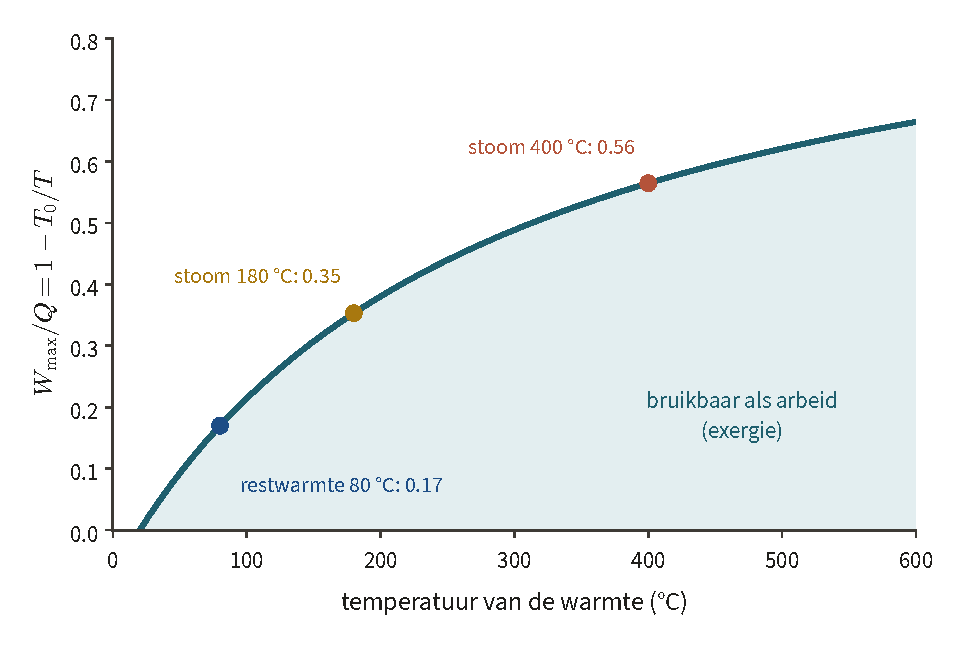
\includegraphics[width=0.7\linewidth]{Figuren/carnotfactor}
    \caption{Maximaal bruikbaar deel van warmte (de Carnotfactor $1 - T_0/T$) in functie van de temperatuur waarbij ze beschikbaar is, voor een omgeving van \SI{20}{\celsius}. Stoom van \SI{400}{\celsius} is voor meer dan de helft omzetbaar in arbeid, restwarmte van \SI{80}{\celsius} voor minder dan een vijfde.}
    \label{fig:carnotfactor}
\end{figure}

\begin{casusuitgewerkt}{gasketel of warmtepomp?}
\emph{Stap 1: de twee routes.} De gasketel levert \SI{0.95}{\kilo\watt\hour} warmte. Via de centrale en een warmtepomp met COP 4 komt er $0.55 \times 4 = \SI{2.2}{\kilo\watt\hour}$ warmte in huis, meer dan het dubbele, ook al gaat in de centrale \SI{45}{\percent} van de energie als restwarmte verloren.

\emph{Stap 2: waarom kan dat?} Kijk naar de exergie. Verbrandingsgassen van zo'n \SI{1500}{\celsius} hebben een Carnotfactor $1 - 278/1773 = 0.84$: bijna alle energie is bruikbaar als arbeid. Water van \SI{35}{\celsius} heeft bij een buitentemperatuur van \SI{5}{\celsius} slechts $1 - 278/308 = 0.10$. De gasketel zet dus hoogwaardige energie om in laagwaardige warmte, en vernietigt daarbij bijna alle exergie, ook al gaat er geen energie verloren. De warmtepomp doet het omgekeerde: ze gebruikt een beetje hoogwaardige energie (elektriciteit, zuivere exergie) om veel laagwaardige warmte uit de buitenlucht op te waarderen.

\emph{Besluit.} Energie gaat nooit verloren, maar haar kwaliteit wel. Wie energie zuinig wil gebruiken, moet de temperatuur van de warmte afstemmen op haar toepassing: hoge temperatuur voor arbeid en processen, lage temperatuur voor verwarming.

\emph{Volgende vraag.} In de buitenunit moet het koelmiddel verdampen bij ongeveer \SI{-5}{\celsius}, onder de temperatuur van de buitenlucht. Waarom kookt de ene stof bij \SI{-42}{\celsius} en de andere bij \SI{100}{\celsius}, en hoe voorspel je dat?
\end{casusuitgewerkt}


\section{De derde hoofdwet van de thermodynamica}
\label{sec:derde-hoofdwet}

Om de entropie van een reactie te berekenen zoals in het voorbeeld van de waterbalans, heb je de entropie van elke stof nodig. Bij de enthalpie konden we enkel verschillen meten, en kozen we een nulpunt per afspraak: $\Delta_fH^\circ = 0$ voor de elementen. Voor entropie blijkt dat niet nodig.

\paragraph{De waarneming.} Walther Nernst mat rond 1906 reacties tussen vaste stoffen bij steeds lagere temperaturen, en stelde vast dat hun reactie-entropie naar nul ging naarmate $T$ naar het absolute nulpunt daalde. Planck trok daaruit de conclusie dat de entropie van elke zuivere, perfect kristallijne stof zelf naar nul gaat.

\begin{definitie}{Derde hoofdwet van de thermodynamica}
De entropie van een perfect kristal van een zuivere stof nadert nul als $T \to \SI{0}{\kelvin}$.
\end{definitie}

Met Boltzmann is dat onmiddellijk duidelijk: in een perfect kristal bij \SI{0}{\kelvin} zit elk atoom op zijn vaste plaats in de laagste energietoestand. Er is precies \'e\'en microtoestand, dus $S = k_B\ln 1 = 0$.

\paragraph{Absolute entropie meten.} Daarmee bestaat er voor entropie een \emph{absolute} schaal. Om de entropie van een stof bij \SI{298}{\kelvin} te kennen, meet men in een calorimeter haar warmtecapaciteit van enkele kelvin tot kamertemperatuur, en telt men alle stukken op, zoals in het voorbeeld van ijs tot stoom:
\[
S_m(T) = \int_0^{T}\frac{C_p}{T}\,\dd T + \sum \frac{\Delta H_\text{trans}}{T_\text{trans}} .
\]
Het allerlaatste stukje, onder de laagste meettemperatuur, wordt geschat met de wet van Debye, $C_p \propto T^3$. De waarde bij \SI{298.15}{\kelvin} en \SI{1}{\bar} heet de \emph{standaardmolaire entropie} $S_m^\circ$ (tabel~\ref{tab:standaardentropie}). Let op: ook een element heeft bij kamertemperatuur een positieve $S_m^\circ$, door translatie, rotatie en vibratie van zijn moleculen (\S~\ref{sec:moleculaire-beweging}), terwijl zijn $\Delta_fH^\circ$ per afspraak nul is.

Niet elke stof is bij \SI{0}{\kelvin} een perfect kristal. In vast koolstofmonoxide kan elke molecule als CO of als OC in het rooster liggen, omdat beide uiteinden bijna even groot zijn. Met twee keuzes per molecule blijft er bij \SI{0}{\kelvin} een \emph{restentropie} $R\ln 2 = \SI{5.8}{\joule\per\mole\per\kelvin}$ over; gemeten wordt \SI{4.6}{\joule\per\mole\per\kelvin}, omdat de ori\"entaties niet helemaal willekeurig zijn. Een mooie bevestiging dat de entropie van Clausius en die van Boltzmann dezelfde grootheid zijn.

\begin{table}[htb]
\centering
\caption{Standaardmolaire entropie $S_m^\circ$ (\SI{298.15}{\kelvin}, \SI{1}{\bar}) voor de stoffen van de ammoniaksynthese. Bron: NIST Chemistry WebBook, NIST Standard Reference Database 69.}
\label{tab:standaardentropie}
\begin{tabular}{lc}
\toprule
Stof & $S_m^\circ$ (\si{\joule\per\mole\per\kelvin}) \\
\midrule
$\mathrm{N_2(g)}$ & 191.6 \\
$\mathrm{H_2(g)}$ & 130.7 \\
$\mathrm{NH_3(g)}$ & 192.8 \\
\bottomrule
\end{tabular}
\end{table}

De reactie-entropie volgt, net als de reactie-enthalpie met de wet van Hess, uit
\begin{equation}
\boxed{\Delta_r S^\circ = \sum_i \nu_i\,S_{m,i}^\circ}
\label{eq:reactie-entropie}
\end{equation}
met $\nu_i$ positief voor producten en negatief voor reagentia.

\begin{voorbeeld}{Reactie-entropie van de ammoniaksynthese}
Voor \ce{N2(g) + 3 H2(g) <=> 2 NH3(g)} geeft tabel~\ref{tab:standaardentropie}:
\[
\Delta_r S^\circ = 2(192.8) - [191.6 + 3(130.7)] = 385.6 - 583.7 = \SI{-198.1}{\joule\per\mole\per\kelvin}.
\]
Sterk negatief: vier mol gas worden er twee, met veel minder bewegingsvrijheid. Een vuistregel die je hier ziet: de entropieverandering van een reactie wordt bijna volledig bepaald door de verandering van het aantal mol gas. Elke mol gas die verdwijnt, kost ongeveer \SI{100}{\joule\per\kelvin}. In de volgende sectie zien we wat dat betekent voor de temperatuur waarbij de ammoniakreactor kan werken.
\end{voorbeeld}

\section{De Gibbs-vrije energie en het thermodynamisch evenwicht}
\label{sec:gibbs}

\begin{casus}{bij welke temperatuur kookt het koelmiddel?}
Moderne warmtepompen gebruiken propaan (R290) als koelmiddel. Bij \SI{1}{\bar} is de verdampingsenthalpie van propaan \SI{19.0}{\kilo\joule\per\mole} en de verdampingsentropie \SI{82}{\joule\per\mole\per\kelvin}. Bij welke temperatuur kookt het? En is dat geschikt om warmte op te nemen uit buitenlucht van \SI{5}{\celsius}?

\emph{Schat eerst zelf:} verdampen kost enthalpie, maar levert entropie op. Bij lage temperatuur wint de enthalpie, bij hoge de entropie. Waar ligt het kantelpunt?
\end{casus}


\subsection{De ingenieursvisie: het systeem en zijn omgeving}

Bij de tweede hoofdwet moesten we telkens de entropie van het universum berekenen: het systeem plus de omgeving. Voor de natuur bestaat er geen grens tussen beide, maar voor een ingenieur wel. Hij kent zijn reactor, kolom of warmtewisselaar goed: de samenstelling, de temperatuur, de druk. Van de omgeving weet hij veel minder: waar gaat de warmte precies heen, en wat gebeurt er daar mee?

Daar zit een praktisch probleem. De richting van een proces wordt bepaald door een grootheid van het hele universum, terwijl de ingenieur enkel het systeem kent. De vraag is dus of er een grootheid bestaat die je volledig uit eigenschappen van het \emph{systeem} kan berekenen, maar die toch zegt in welke richting het proces loopt. Josiah Willard Gibbs toonde in 1876 dat dat kan, voor het geval dat in de chemie en procestechniek bijna altijd geldt: constante temperatuur en constante druk.

\subsection{De Gibbs-vrije energie}

\begin{definitie}{Gibbs-vrije energie}
\begin{equation}
G = H - TS.
\end{equation}
Bij constante temperatuur en druk geldt: $\Delta G < 0$ spontaan, $\Delta G = 0$ evenwicht, $\Delta G > 0$ niet spontaan (de omgekeerde richting is dan spontaan).
\end{definitie}

$G$ is geen nieuwe vorm van energie. Het is een slim gekozen combinatie van grootheden die we al kennen, die de omgeving ongemerkt meerekent. Dat zien we in de afleiding.

\subsubsection{Afleiding uit de tweede hoofdwet}

We vertrekken van de tweede hoofdwet en werken de omgeving weg, in vier stappen.
\begin{enumerate}
\item \emph{Splits het universum.} Voor een klein stapje van het proces eist de tweede hoofdwet
\[
\dd S_\text{univ} = \dd S + \dd S_\text{omg} \geq 0,
\]
met $\dd S$ de entropieverandering van het systeem.
\item \emph{Druk de omgeving uit in het systeem.} Bij constante druk is de warmte die het systeem opneemt gelijk aan $\dd H$ (hoofdstuk~\ref{ch:energie}). De omgeving ontvangt dus $-\dd H$. Ze is een groot reservoir op temperatuur $T$, zodat $\dd S_\text{omg} = -\dd H/T$, zoals bij de lokale entropieafname.
\item \emph{Vul in.} $\dd S - \dd H/T \geq 0$. Nu staan er enkel nog eigenschappen van het systeem.
\item \emph{Vermenigvuldig met $-T$.} Omdat $T > 0$ keert het ongelijkheidsteken om: $\dd H - T\,\dd S \leq 0$. Bij constante temperatuur is $\dd H - T\,\dd S$ precies $\dd(H - TS) = \dd G$, dus
\[
\dd G \leq 0 \qquad (\text{constante } T \text{ en } p).
\]
\end{enumerate}
Een daling van $G$ van het systeem is dus hetzelfde als een stijging van de entropie van het universum: $\Delta G = -T\Delta S_\text{univ}$. De Gibbs-vrije energie is geen nieuwe natuurwet, maar de tweede hoofdwet, herschreven in eigenschappen van het systeem. De term $\Delta H$ staat voor wat er in de omgeving gebeurt, de term $T\Delta S$ voor wat er in het systeem gebeurt.

Het woord ``vrij'' heeft ook een concrete betekenis: $-\Delta G$ is de maximale nuttige arbeid, naast de volumearbeid tegen de atmosfeer, die een proces bij constante $T$ en $p$ kan leveren. Een brandstofcel of batterij zet $-\Delta G$ om in elektrische arbeid (hoofdstuk~\ref{ch:elektrochemie}), niet $-\Delta H$.

\begin{voorbeeld}{Werkt de ammoniakreactor bij elke temperatuur?}
Voor \ce{N2 + 3 H2 -> 2 NH3} is $\Delta_r H^\circ = \SI{-92.2}{\kilo\joule\per\mole}$ (hoofdstuk~\ref{ch:energie}) en $\Delta_r S^\circ = \SI{-198.1}{\joule\per\mole\per\kelvin}$. Bij \SI{298}{\kelvin}:
\[
\Delta_r G^\circ = \Delta_r H^\circ - T\Delta_r S^\circ = -92.2 - (298)(-0.1981) = -92.2 + 59.0 = \SI{-33.2}{\kilo\joule\per\mole}.
\]
De reactie is bij kamertemperatuur spontaan. De twee termen werken echter tegen elkaar: de enthalpie is gunstig, de entropie ongunstig. Bij hogere temperatuur weegt de entropieterm zwaarder, en bij
\[
T^* = \frac{\Delta_r H^\circ}{\Delta_r S^\circ} = \frac{-92\,200}{-198.1} = \SI{465}{\kelvin} \approx \SI{190}{\celsius}
\]
wordt $\Delta_r G^\circ$ nul. De katalysator werkt pas goed bij 400 tot \SI{500}{\celsius}, ruim boven $T^*$: daar is $\Delta_r G^\circ$ positief. Dat de fabriek toch ammoniak maakt, komt door de hoge druk van \SI{200}{\bar}. Hoe druk en temperatuur samen de opbrengst bepalen, is het onderwerp van hoofdstuk~\ref{ch:reagerend}.
\end{voorbeeld}

\subsubsection{De fundamentele vergelijkingen}
\label{sec:fundamentele-vgl}

Hoe verandert $G$ als je de temperatuur of de druk verandert? Dat volgt uit de combinatie van de eerste en de tweede hoofdwet. We bouwen het op in drie stappen, telkens met de productregel.

\paragraph{Stap 1: de interne energie.} Voor een gesloten systeem dat enkel volumearbeid uitwisselt, geeft de eerste hoofdwet voor een reversibele verandering $\dd U = \delta Q_\text{rev} - p\,\dd V$. Met Clausius is $\delta Q_\text{rev} = T\,\dd S$:
\begin{equation}
\boxed{\dd U = T\,\dd S - p\,\dd V}
\label{eq:fundU}
\end{equation}
We leidden dit af langs een reversibele weg, maar het geldt voor elke verandering: $U$, $S$ en $V$ zijn toestandsfuncties, en het verband tussen hun veranderingen hangt niet af van hoe je van de ene toestand naar de andere gaat.

\paragraph{Stap 2: de enthalpie.} Met $H = U + pV$ geeft de productregel $\dd H = \dd U + p\,\dd V + V\,\dd p$. Vul vergelijking~\eqref{eq:fundU} in:
\begin{equation}
\dd H = (T\,\dd S - p\,\dd V) + p\,\dd V + V\,\dd p = T\,\dd S + V\,\dd p.
\label{eq:fundH}
\end{equation}

\paragraph{Stap 3: de Gibbs-vrije energie.} Met $G = H - TS$ geeft de productregel $\dd G = \dd H - T\,\dd S - S\,\dd T$. Vul vergelijking~\eqref{eq:fundH} in:
\[
\dd G = (T\,\dd S + V\,\dd p) - T\,\dd S - S\,\dd T,
\]
zodat
\begin{equation}\label{eq:fundG}
\boxed{\dd G = V\,\dd p - S\,\dd T}
\end{equation}

\paragraph{Wat zegt deze vergelijking?} Ze geeft twee concrete regels.
\begin{itemize}
\item Bij constante druk is $(\partial G/\partial T)_p = -S$. Warm je een stof op, dan daalt haar $G$, en sneller naarmate haar entropie groter is. Een gas daalt dus sneller dan een vloeistof, en een vloeistof sneller dan een vaste stof. Daarom wint bij hoge temperatuur altijd de fase met de hoogste entropie (\S\ref{sec:mu-p-T}).
\item Bij constante temperatuur is $(\partial G/\partial p)_T = V$. Verhoog je de druk, dan stijgt $G$, en sterker naarmate het volume groter is. Voor een gas is dat effect groot, voor een vloeistof of vaste stof klein. Daarom verschuift hoge druk een evenwicht naar de kant met minder mol gas, zoals bij de ammoniaksynthese.
\end{itemize}
In hoofdstuk~\ref{ch:niet-reagerend} levert vergelijking~\eqref{eq:fundG} de chemische potentiaal als functie van druk en samenstelling, en in hoofdstuk~\ref{ch:reagerend} de vergelijking van Van 't Hoff.

\subsection{De competitie tussen enthalpie en entropie}

In $\Delta G = \Delta H - T\Delta S$ trekken twee tendensen aan het systeem. Het wil zijn enthalpie verlagen: sterke bindingen en gunstige intermoleculaire interacties. En het wil naar toestanden met meer microtoestanden: hogere entropie. De temperatuur bepaalt het gewicht van de tweede tendens. Bij lage $T$ beslist vooral $\Delta H$, bij hoge $T$ vooral $\Delta S$. Volgens de tekens van $\Delta H$ en $\Delta S$ zijn er vier gevallen (figuur~\ref{fig:dG-temperatuur}):
\begin{itemize}
\item $\Delta H < 0$ en $\Delta S > 0$: altijd spontaan (ontbinding van waterstofperoxide);
\item $\Delta H > 0$ en $\Delta S < 0$: nooit spontaan (ozon vormen uit zuurstof);
\item $\Delta H < 0$ en $\Delta S < 0$: spontaan \emph{onder} $T^* = \Delta H/\Delta S$ (ammoniaksynthese, bevriezen);
\item $\Delta H > 0$ en $\Delta S > 0$: spontaan \emph{boven} $T^*$ (kalk branden, smelten, verdampen).
\end{itemize}

\begin{figure}[htb]
    \centering
    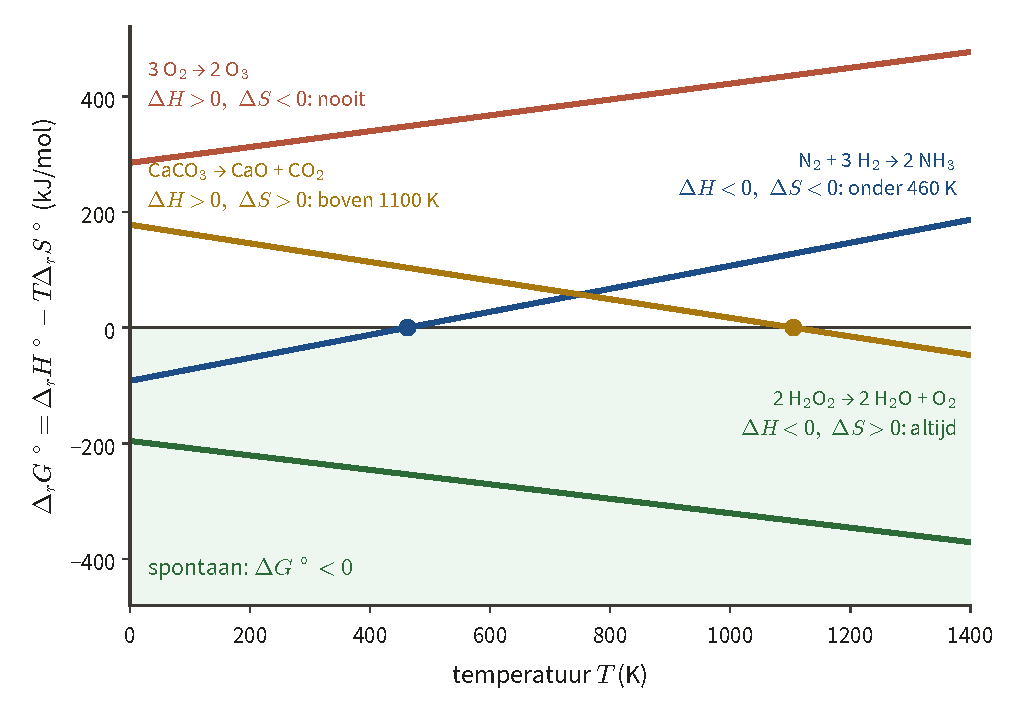
\includegraphics[width=0.75\linewidth]{Figuren/dG_temperatuur}
    \caption{$\Delta_r G^\circ$ in functie van de temperatuur voor vier reacties, \'e\'en per tekencombinatie van $\Delta_r H^\circ$ en $\Delta_r S^\circ$. De helling is $-\Delta_r S^\circ$, het snijpunt met de verticale as $\Delta_r H^\circ$. De bolletjes markeren $T^* = \Delta_r H^\circ/\Delta_r S^\circ$, waar de reactie van richting wisselt (standaardwaarden bij \SI{298}{\kelvin}, constant verondersteld).}
    \label{fig:dG-temperatuur}
\end{figure}

\begin{voorbeeld}{De smelttemperatuur van water}
Bij het smelten van ijs moeten waterstofbruggen gedeeltelijk worden verbroken. Dat kost energie: $\Delta H_\text{fus} = \SI{6.01}{\kilo\joule\per\mole}$, de omgeving moet warmte leveren en haar entropie daalt. Tegelijk krijgen de watermoleculen in de vloeistof veel meer bewegingsvrijheid: $\Delta S_\text{fus} = \SI{22.0}{\joule\per\mole\per\kelvin}$. Welke tendens wint, hangt af van de temperatuur:
\begin{itemize}
\item bij \SI{-10}{\celsius}: $\Delta G_\text{fus} = 6010 - (263)(22.0) = \SI{+224}{\joule\per\mole}$, ijs blijft ijs;
\item bij \SI{+10}{\celsius}: $\Delta G_\text{fus} = 6010 - (283)(22.0) = \SI{-216}{\joule\per\mole}$, ijs smelt;
\item het kantelpunt ligt waar $\Delta G_\text{fus} = 0$: $T_\text{fus} = \Delta H_\text{fus}/\Delta S_\text{fus} = 6010/22.0 = \SI{273}{\kelvin}$.
\end{itemize}
Het smeltpunt is dus precies de temperatuur waar enthalpie en entropie elkaar in evenwicht houden. Bij lage temperatuur weegt de entropiewinst te licht om de smeltwarmte te betalen; bij hoge temperatuur wint ze.
\end{voorbeeld}

\subsection{Spontaniteit is niet snelheid}

Spontaniteit zegt iets over de \emph{richting}, niet over de \emph{snelheid}. Diamant zou spontaan in grafiet moeten overgaan ($\Delta G < 0$), maar bij kamertemperatuur gebeurt dat in geen miljard jaar. Methaan en zuurstof kunnen jarenlang samen in een tank zitten; pas een vonk zet de verbranding in gang. Hoe snel een spontaan proces verloopt, is het onderwerp van de kinetiek (hoofdstuk~\ref{ch:kinetiek}).

\subsection{Het thermodynamisch evenwicht}

Een systeem bij constante $T$ en $p$ evolueert zoals een bal in een berglandschap: bergaf in $G$, tot in de vallei. In dat minimum is er geen drijvende kracht meer: het systeem is in evenwicht. Voor fase-evenwichten en mengsels werken we dat uit in hoofdstuk~\ref{ch:niet-reagerend}, voor chemische reacties in hoofdstuk~\ref{ch:reagerend}.

\begin{casusuitgewerkt}{bij welke temperatuur kookt het koelmiddel?}
Verdampen is spontaan zodra $\Delta G_\text{vap} = \Delta H_\text{vap} - T\Delta S_\text{vap} < 0$. Het kookpunt is de temperatuur waarbij beide termen elkaar opheffen:
\[
T_b = \frac{\Delta H_\text{vap}}{\Delta S_\text{vap}} = \frac{19\,000}{82} = \SI{232}{\kelvin} = \SI{-41}{\celsius}.
\]
Gemeten: \SI{-42}{\celsius}. Bij \SI{1}{\bar} kookt propaan dus ruim onder de buitentemperatuur: het neemt gretig warmte op uit lucht van \SI{5}{\celsius}, zelfs uit lucht van \SI{-20}{\celsius}. In de buitenunit werkt men bij een iets hogere druk, ongeveer \SI{4}{\bar}, zodat het kookpunt naar \SI{-5}{\celsius} schuift; hoe het kookpunt met de druk verandert, volgt in hoofdstuk~\ref{ch:niet-reagerend}. In de condensor perst de compressor het koelmiddel tot ongeveer \SI{12}{\bar}, waar het pas bij zo'n \SI{35}{\celsius} condenseert en zijn warmte aan de vloerverwarming afgeeft.

De verdampingsentropie van \SI{82}{\joule\per\mole\per\kelvin} is geen toeval: bijna alle vloeistoffen winnen bij verdampen ongeveer evenveel microtoestanden (regel van Trouton, hoofdstuk~\ref{ch:intermoleculair}). Een koelmiddel kies je dus vooral via zijn verdampingsenthalpie, dus via de sterkte van de krachten tussen zijn moleculen.
\end{casusuitgewerkt}


\section{De chemische potentiaal}
\label{sec:chemische-potentiaal}

Tot nu toe bekeken we een systeem als geheel. Processen bevatten echter zelden \'e\'en zuivere stof. In een reactor, een destillatiekolom of een absorber verandert de hoeveelheid van elke component afzonderlijk: ammoniak ontstaat, ethanol verdampt sneller dan water, \ce{CO2} lost op in een solvent. We hebben dus een drijvende kracht \emph{per component} nodig.

\paragraph{Een potentiaal voor materie.} Elke spontane stroom in de natuur wordt gedreven door een verschil in een potentiaal, en stopt wanneer dat verschil verdwijnt:
\begin{center}
\begin{tabular}{lll}
\toprule
wat stroomt & drijvende kracht & evenwicht als \\
\midrule
water in een rivier & hoogteverschil & gelijke hoogte \\
elektrische lading & spanningsverschil & gelijke potentiaal \\
warmte & temperatuurverschil & gelijke $T$ \\
een fluïdum & drukverschil & gelijke $p$ \\
materie (diffusie, faseovergang, reactie) & verschil in chemische potentiaal & gelijke $\mu$ \\
\bottomrule
\end{tabular}
\end{center}

\paragraph{Definitie.} De chemische potentiaal van component $i$ is
\begin{equation}
\mu_i = \left(\frac{\partial G}{\partial n_i}\right)_{T,p,n_{j\neq i}} .
\end{equation}
In woorden: met hoeveel stijgt de Gibbs-vrije energie van het systeem als je een kleine hoeveelheid van component $i$ toevoegt, bij constante temperatuur, druk en hoeveelheden van de andere componenten? Voor een zuivere stof is dat gewoon de molaire Gibbs-vrije energie, $\mu = G_m$.

\paragraph{Waarom stroomt materie naar lage $\mu$?} Stel dat \SI{1}{\milli\mole} van component $i$ overgaat van fase $\alpha$ naar fase $\beta$, bijvoorbeeld van vloeistof naar damp. De Gibbs-vrije energie van fase $\alpha$ daalt met $\mu_i^\alpha \times \SI{1}{\milli\mole}$, die van fase $\beta$ stijgt met $\mu_i^\beta \times \SI{1}{\milli\mole}$. Samen is $\dd G = (\mu_i^\beta - \mu_i^\alpha)\,\dd n_i$. Volgens het criterium $\dd G < 0$ gebeurt dat enkel vanzelf als $\mu_i^\beta < \mu_i^\alpha$. Een component verplaatst zich dus spontaan van hoge naar lage chemische potentiaal, net zoals warmte van hoge naar lage temperatuur.

\paragraph{Het criterium voor evenwicht.} De overgang stopt wanneer $\mu_i^\alpha = \mu_i^\beta$: dan levert een verschuiving geen daling van $G$ meer op. In evenwicht is de chemische potentiaal van elke component overal gelijk. Water in een gesloten vat is in evenwicht met zijn damp als $\mu^\text{vloeistof} = \mu^\text{damp}$; een opgeloste stof diffundeert tot $\mu$ overal gelijk is; een reactie loopt tot de chemische potentialen van reagentia en producten, gewogen met hun stoichiometrische co\"effici\"enten, in balans zijn.

Hoe $\mu$ verandert met de temperatuur, de druk en de samenstelling van een mengsel, waarom het smeltpunt en het kookpunt precies de punten zijn waar twee fasen dezelfde $\mu$ hebben, en hoe je zo dampdrukken, oplosbaarheden en evenwichtsconstanten berekent, volgt in hoofdstuk~\ref{ch:niet-reagerend} (fase-evenwichten en mengsels) en hoofdstuk~\ref{ch:reagerend} (chemische evenwichten).

\section{De warmtepomp opnieuw bekeken}

Met de begrippen uit dit hoofdstuk kan je de vragen uit het begin beantwoorden:
\begin{itemize}
\item \emph{Waarom warmte niet vanzelf naar binnen stroomt} (\S\ref{sec:waarschijnlijkheid-entropie}): een gelijkmatige verdeling van de energie heeft overweldigend veel meer microtoestanden. De entropie, $S = k_B\ln\Omega$, meet dat aantal, en de tweede hoofdwet zegt dat ze in totaal nooit daalt.
\item \emph{Hoeveel stroom} (\S\ref{sec:tweedehoofdwet}): uit de entropiebalans volgt $\mathrm{COP} \leq T_\mathrm{h}/(T_\mathrm{h} - T_\mathrm{c})$. Voor vloerverwarming bij \SI{5}{\celsius} buiten is dat 10, in de praktijk ongeveer 4. Dezelfde redenering geeft de minimale arbeid voor de koelmachine van de ammoniakfabriek: \SI{2.3}{\mega\watt}.
\item \emph{Gasketel of warmtepomp} (\S\ref{sec:exergie}): niet de hoeveelheid energie telt, maar haar kwaliteit. Gas verbranden voor water van \SI{35}{\celsius} vernietigt bijna alle exergie; via elektriciteit en een warmtepomp komt er twee keer meer warmte in huis.
\item \emph{Het koelmiddel} (\S\ref{sec:gibbs}): de stof kookt waar $\Delta G_\text{vap} = 0$, dus bij $T_b = \Delta H_\text{vap}/\Delta S_\text{vap}$. Hetzelfde criterium, $\Delta G < 0$, bepaalt of een reactie vanzelf verloopt.
\end{itemize}
Het criterium $\Delta G \leq 0$, of in een mengsel gelijke chemische potentialen, is de rode draad van de volgende hoofdstukken: fase-evenwichten en mengsels (hoofdstuk~\ref{ch:niet-reagerend}), chemische evenwichten (hoofdstuk~\ref{ch:reagerend}) en elektrochemie (hoofdstuk~\ref{ch:elektrochemie}).

\newpage
\section{Oefeningen}

% Oefeningen bij dit hoofdstuk (ingevoegd achteraan het hoofdstuk met \input).
% Een oefening:  \begin{oefening}[titel] ... \end{oefening}   (boek en website)
% De oplossing:  \begin{oplossing} ... \end{oplossing}       (enkel website, dichtgeklapt)

Neem $R = \SI{8.314}{\joule\per\mole\per\kelvin}$ en $p^\circ = \SI{1}{\bar}$.

\begin{oefening}[Mengentropie van een driecomponent-mengsel]
Een vat bevat aanvankelijk \(1\,\mathrm{mol}\) stikstof, \(1\,\mathrm{mol}\) zuurstof en \(1\,\mathrm{mol}\) argon, elk in afzonderlijke compartimenten bij gelijke temperatuur en druk. De compartimenten worden geopend en de gassen mengen spontaan.

\begin{enumerate}
\item[(a)]
  Bereken de mengentropie per mol mengsel.
\item[(b)]
  Bereken de bijbehorende verandering van de Gibbs-vrije energie bij \(298\,\mathrm{K}\).
\item[(c)]
  Hoeveel minimale arbeid is nodig om het mengsel bij \(298\,\mathrm{K}\) terug te scheiden in de drie zuivere componenten?
\end{enumerate}

\emph{Hint:} \(\Delta S_{\text{meng}} = -R\sum_i x_i \ln x_i\); \(\Delta G_{\text{meng}} = -T \Delta S_{\text{meng}}\) voor ideale mengsels.
\end{oefening}
\begin{oplossing}
\textbf{Resultaat:} (a) \(\Delta S_{\text{meng}}\) = \textbf{9.13 J/(mol\ensuremath{\cdot{}}K)} (27.4 J/K in totaal). (b) \(\Delta G_{\text{meng}}\) = \textbf{\ensuremath{-}2.72 kJ/mol} (\ensuremath{-}8.17 kJ). (c) \(W_{\min}\) = \textbf{8.17 kJ}.

\textbf{(a)} Met \(x_i = 1/3\): \(\Delta S_{\text{meng}} = -R \cdot 3 \cdot \frac{1}{3}\ln\frac{1}{3} = R\ln 3 = 9.13\,\mathrm{J/(mol\cdot K)}\) per mol mengsel, of \(27.4\,\mathrm{J/K}\) voor de 3 mol samen.

\textbf{(b)} \(\Delta G_{\text{meng}} = -T\Delta S_{\text{meng}} = -(298)(9.13) = -2.72\,\mathrm{kJ/mol}\) mengsel, of \(-8.17\,\mathrm{kJ}\) in totaal. Negatief: mengen verloopt spontaan.

\textbf{(c)} Scheiden is het omgekeerde proces met \(\Delta G = +8.17\,\mathrm{kJ}\). De minimale (reversibele) arbeid bedraagt dus \(8.17\,\mathrm{kJ}\). Echte scheidingsprocessen (cryogene luchtscheiding, membranen) verbruiken daar een veelvoud van; deze ondergrens toont hoeveel ruimte er theoretisch is voor energiebesparing.
\end{oplossing}

\begin{oefening}[Entropie bij faseovergangen]
Thallium smelt bij \(304\,^\circ\mathrm{C}\) met een smeltenthalpie van \(\Delta H_{\text{fus}} = 4.27\,\mathrm{kJ/mol}\).

\begin{enumerate}
\item[(a)]
  Bereken de smeltentropie.
\item[(b)]
  Verklaar vanuit de orde-grootte waarom deze entropie kleiner is dan de verdampingsentropie van water (\(\Delta S_{\text{vap}} \approx 109\,\mathrm{J/(mol\cdot K)}\)).
\item[(c)]
  Bereken de verandering van de Gibbs-vrije energie bij het smelten precies op het smeltpunt.
\end{enumerate}
\end{oefening}
\begin{oplossing}
\textbf{Resultaat:} (a) \(\Delta S_{\text{fus}}\) = \textbf{7.40 J/(mol\ensuremath{\cdot{}}K)}. (c) Op het smeltpunt is \(\Delta G_{\text{fus}}\) = \textbf{0}.

\textbf{(a)} \(\Delta S_{\text{fus}} = \Delta H_{\text{fus}}/T_{\text{fus}} = 4270/577.15 = 7.40\,\mathrm{J/(mol\cdot K)}\).

\textbf{(b)} Bij smelten blijven de atomen dicht opeengepakt: de vloeistof is slechts iets wanordelijker dan het kristal, zodat het aantal toegankelijke microtoestanden weinig toeneemt. Bij verdampen neemt het beschikbare volume per molecule met een factor duizend toe, en bij water wordt bovendien het geordende waterstofbrugnetwerk verbroken. Daarom is \(\Delta S_{\text{vap}}\) typisch een grootteorde groter dan \(\Delta S_{\text{fus}}\).

\textbf{(c)} Op het smeltpunt zijn vaste stof en vloeistof in evenwicht: \(\Delta G_{\text{fus}} = \Delta H_{\text{fus}} - T_{\text{fus}}\Delta S_{\text{fus}} = 0\).
\end{oplossing}

\begin{oefening}[Spontaniteitscriterium: smelten van ijs bij verschillende temperaturen]
Voor het smelten van ijs geldt \(\Delta H_{\text{fus}} = 6.0\,\mathrm{kJ/mol}\) en \(\Delta S_{\text{fus}} = 22.0\,\mathrm{J/(mol\cdot K)}\) (verondersteld constant).

\begin{enumerate}
\item[(a)]
  Bereken \(\Delta G\) bij \(-10\,^\circ\mathrm{C}\), \(0\,^\circ\mathrm{C}\) en \(+10\,^\circ\mathrm{C}\).
\item[(b)]
  Bepaal bij welke temperatuur ijs en vloeibaar water in evenwicht zijn.
\item[(c)]
  Verklaar vanuit het teken van \(\Delta G\) waarom ijs bij \(-10\,^\circ\mathrm{C}\) niet spontaan smelt.
\end{enumerate}
\end{oefening}
\begin{oplossing}
\textbf{Resultaat:} (a) \(\Delta G\) = \textbf{+211}, \textbf{\ensuremath{\approx{}} 0} en \textbf{\ensuremath{-}229 J/mol} bij 263, 273 en 283 K. (b) \(T\) = \textbf{272.7 K} (\ensuremath{\approx{}} 0 °C). (c) Bij \ensuremath{-}10 °C is \textbf{bevriezen} spontaan.

\textbf{(a)} Met \(\Delta G = \Delta H - T\Delta S\):

\begin{center}
\begin{tabular}{ll}
\toprule
\(T\) & \(\Delta G\) (J/mol) \\
\midrule
\(263.15\,\mathrm{K}\) & \(+211\) \\
\(273.15\,\mathrm{K}\) & \(-9\) (\ensuremath{\approx{}} 0) \\
\(283.15\,\mathrm{K}\) & \(-229\) \\
\bottomrule
\end{tabular}
\end{center}

\textbf{(b)} \(\Delta G = 0\) bij \(T = \Delta H/\Delta S = 6000/22.0 = 272.7\,\mathrm{K}\), of \(-0.4\,^\circ\mathrm{C}\). Het kleine verschil met \(0\,^\circ\mathrm{C}\) komt door de afronding van de gegevens.

\textbf{(c)} Bij \(-10\,^\circ\mathrm{C}\) is \(\Delta G > 0\): de enthalpiekost van het smelten weegt zwaarder dan de entropiewinst \(T\Delta S\). Het omgekeerde proces, bevriezen, is dan spontaan. Daarom strooit men zout op wegen: zout verlaagt de chemische potentiaal van het vloeibare water (hoofdstuk 5), waardoor het smeltpunt daalt.
\end{oplossing}

\begin{oefening}[Evenwichtsconstante en standaardreactie-Gibbsenergie]
Voor de reactie

\[
\mathrm{N_2O_4(g) \rightleftharpoons 2\,NO_2(g)}
\]

bedraagt \(\Delta_r G^\circ = +4.8\,\mathrm{kJ/mol}\) bij \(298\,\mathrm{K}\).

\begin{enumerate}
\item[(a)]
  Bereken de evenwichtsconstante \(K\) bij \(298\,\mathrm{K}\).
\item[(b)]
  Is de reactie bij standaardomstandigheden spontaan in de voorwaartse richting?
\item[(c)]
  Bij welke waarde van het reactiequotiënt \(Q\) zou de reactie precies in evenwicht zijn?
\end{enumerate}
\end{oefening}
\begin{oplossing}
\textbf{Resultaat:} (a) \(K\) = \textbf{0.144}. (b) \textbf{Nee}, bij \(Q = 1\) verloopt de reactie naar links. (c) Evenwicht bij \(Q = K\) = \textbf{0.144}.

\textbf{(a)} \(K = \exp(-\Delta_r G^\circ/RT) = \exp\!\left(-\dfrac{4800}{(8.314)(298)}\right) = 0.144\).

\textbf{(b)} Nee. Bij standaardomstandigheden (beide gassen bij \(1\,\mathrm{bar}\), dus \(Q = 1\)) is \(\Delta_r G = \Delta_r G^\circ > 0\): de reactie verloopt spontaan in de \emph{omgekeerde} richting tot het evenwicht bereikt is. Dat betekent niet dat er geen \(\mathrm{NO_2}\) gevormd wordt: vertrekkend van zuiver \(\mathrm{N_2O_4}\) (\(Q = 0\)) dissocieert een deel wel degelijk.

\textbf{(c)} Evenwicht wanneer \(\Delta_r G = \Delta_r G^\circ + RT\ln Q = 0\), dus \(Q = K = 0.144\).
\end{oplossing}

\begin{oefening}[Invloed van temperatuur: de vergelijking van Van 't Hoff]
Voor de ammoniaksynthese \(\mathrm{N_2 + 3\,H_2 \rightleftharpoons 2\,NH_3}\) bedraagt \(\Delta_r H^\circ = -92.4\,\mathrm{kJ/mol}\) en \(\Delta_r G^\circ = -33.0\,\mathrm{kJ/mol}\) bij \(298\,\mathrm{K}\).

\begin{enumerate}
\item[(a)]
  Bereken \(K\) bij \(298\,\mathrm{K}\).
\item[(b)]
  Schat \(K\) bij \(700\,\mathrm{K}\) (veronderstel \(\Delta_r H^\circ\) constant). Gebruik de geïntegreerde vorm van Van 't Hoff.
\item[(c)]
  Verklaar vanuit het teken van \(\Delta_r H^\circ\) waarom de evenwichtsconstante daalt bij stijgende temperatuur.
\item[(d)]
  Combineer met Hoofdstuk 1: bereken ook \(\Delta_r S^\circ\) bij \(298\,\mathrm{K}\).
\end{enumerate}
\end{oefening}
\begin{oplossing}
\textbf{Resultaat:} (a) \(K_{298}\) = \textbf{6.1\ensuremath{\cdot{}}10\ensuremath{^{5}}}. (b) \(K_{700}\) = \textbf{3.0\ensuremath{\cdot{}}10\ensuremath{^{-4}}}. (c) Exotherm: \(K\) \textbf{daalt} met \(T\). (d) \(\Delta_r S^\circ\) = \textbf{\ensuremath{-}199 J/(mol\ensuremath{\cdot{}}K)}.

\textbf{(a)} \(\ln K = 33\,000/(8.314 \times 298) = 13.32\), dus \(K = 6.1\times10^{5}\).

\textbf{(b)}

\[
\ln\frac{K_2}{K_1} = -\frac{-92\,400}{8.314}\left(\frac{1}{700} - \frac{1}{298}\right) = -21.4
\]

zodat \(\ln K_2 = 13.32 - 21.4 = -8.1\) en \(K_2 = 3.0\times10^{-4}\).

\textbf{(c)} Volgens \(\mathrm{d}\ln K/\mathrm{d}T = \Delta_r H^\circ/(RT^2)\) daalt \(\ln K\) met \(T\) wanneer \(\Delta_r H^\circ < 0\). Fysisch: bij een exotherme reactie ``werkt'' extra warmte de vorming van producten tegen (Le Chatelier).

\textbf{(d)} \(\Delta_r S^\circ = (\Delta_r H^\circ - \Delta_r G^\circ)/T = (-92\,400 + 33\,000)/298 = -199\,\mathrm{J/(mol\cdot K)}\), in overeenstemming met de \(-198.1\,\mathrm{J/(mol\cdot K)}\) uit de theorie. Negatief, omdat 4 mol gas omgezet wordt in 2 mol gas.
\end{oplossing}

\begin{oefening}[Le Châtelier: invloed van druk op ammoniaksynthese]
Beschouw opnieuw de ammoniaksynthese. Bij een bepaalde temperatuur bedraagt \(K = 1.0\times10^{-3}\).

\begin{enumerate}
\item[(a)]
  Een reactiemengsel bevat aanvankelijk gelijke molfracties \(\mathrm{N_2}\), \(\mathrm{H_2}\) en \(\mathrm{NH_3}\) bij een totale druk van \(1\,\mathrm{bar}\). Bereken \(Q\) en bepaal de spontane richting.
\item[(b)]
  Hoe verandert \(Q\) wanneer de totale druk wordt verhoogd tot \(200\,\mathrm{bar}\)? Verklaar waarom een drukverhoging de vorming van ammoniak bevordert.
\item[(c)]
  Waarom verandert de evenwichtsconstante \(K\) zelf \emph{niet} met de druk?
\end{enumerate}

\emph{Hint:} bij een gasreactie met afname van aantal mol geldt \(Q \propto p^{\Delta \nu} = 1/p^{|\Delta \nu|}\).
\end{oefening}
\begin{oplossing}
\textbf{Resultaat:} (a) \(Q\) = \textbf{9} \textgreater{} \(K\): ammoniak ontleedt. (b) \(Q\) = \textbf{2.25\ensuremath{\cdot{}}10\ensuremath{^{-4}}} \textless{} \(K\): ammoniak wordt gevormd. (c) \(K\) hangt enkel af van \(T\).

\textbf{(a)} Met \(p_i = x_i p\) en \(p^\circ = 1\,\mathrm{bar}\):

\[
Q = \frac{(x_{\mathrm{NH_3}}p/p^\circ)^2}{(x_{\mathrm{N_2}}p/p^\circ)(x_{\mathrm{H_2}}p/p^\circ)^3} = \frac{x_{\mathrm{NH_3}}^2}{x_{\mathrm{N_2}}x_{\mathrm{H_2}}^3}\left(\frac{p}{p^\circ}\right)^{-2} = \frac{(1/3)^2}{(1/3)^4}(1)^{-2} = 9
\]

\(Q = 9 \gg K\): de reactie verloopt spontaan naar links, ammoniak ontleedt.

\textbf{(b)} De samenstelling blijft dezelfde, maar de drukfactor wordt \((200)^{-2}\): \(Q = 9/40\,000 = 2.25\times10^{-4} < K\). Nu verloopt de reactie spontaan naar rechts. Omdat het aantal mol gas afneemt (\(\Delta\nu = 2 - 4 = -2\)), daalt \(Q\) met de druk als \(p^{\Delta\nu} = p^{-2}\); het evenwicht moet dan naar de kant van de producten schuiven om \(Q\) weer gelijk te maken aan \(K\).

\textbf{(c)} \(K = \exp(-\Delta_r G^\circ/RT)\) is gedefinieerd met de standaardtoestand bij de vaste druk \(p^\circ = 1\,\mathrm{bar}\). Daardoor hangt \(K\) enkel af van de temperatuur. De druk verandert wel \(Q\), en dus de evenwichtssamenstelling.
\end{oplossing}

\begin{oefening}[Geïntegreerde case: Haber--Bosch bij twee temperaturen]
Een ingenieur moet een ammoniakreactor ontwerpen en overweegt twee bedrijfstemperaturen: \(400\,^\circ\mathrm{C}\) en \(500\,^\circ\mathrm{C}\). Voor de synthese \(\mathrm{N_2 + 3\,H_2 \rightleftharpoons 2\,NH_3}\) geldt bij \(298\,\mathrm{K}\): \(\Delta_r H^\circ = -92.4\,\mathrm{kJ/mol}\), \(\Delta_r G^\circ = -33.0\,\mathrm{kJ/mol}\), en \(\Delta_r C_p^\circ \approx -5.2\,\mathrm{J/(mol\cdot K)}\) (constant verondersteld).

\begin{enumerate}
\item[(a)]
  Gebruik de wet van Kirchhoff (Hoofdstuk 1) om \(\Delta_r H^\circ\) te berekenen bij beide temperaturen.
\item[(b)]
  Bereken \(\Delta_r S^\circ\) bij \(298\,\mathrm{K}\) en schat \(\Delta_r S^\circ\) bij \(500\,^\circ\mathrm{C}\) via \(\Delta_r S^\circ(T) = \Delta_r S^\circ(T_0) + \Delta_r C_p^\circ \ln(T/T_0)\).
\item[(c)]
  Bereken \(\Delta_r G^\circ\) bij beide temperaturen via \(G = H - TS\).
\item[(d)]
  Bereken \(K\) bij beide temperaturen.
\item[(e)]
  Concludeer: welke temperatuur levert thermodynamisch de hoogste opbrengst? Leg uit waarom de industrie toch bij \(400\)--\(500\,^\circ\mathrm{C}\) werkt.
\end{enumerate}

\emph{Hint:} deze oefening combineert alle hoofdstukken 1--3: Kirchhoff (H1), enthalpie/entropie/Gibbs (H3), en de brug met de evenwichtsconstante (H3).
\end{oefening}
\begin{oplossing}
\textbf{Resultaat:} Met \(\Delta_r C_p^\circ\) = \ensuremath{-}5.2 J/(mol\ensuremath{\cdot{}}K): \(K\)(673 K) = \textbf{4.9\ensuremath{\cdot{}}10\ensuremath{^{-4}}} en \(K\)(773 K) = \textbf{5.5\ensuremath{\cdot{}}10\ensuremath{^{-5}}}. Lagere \(T\) is thermodynamisch gunstiger; 400--500 °C is een \textbf{compromis met de snelheid}.

Met de gegeven \(\Delta_r C_p^\circ = -5.2\,\mathrm{J/(mol\cdot K)}\):

\begin{center}
\begin{tabular}{lll}
\toprule
 & \(673\,\mathrm{K}\) (\(400\,^\circ\mathrm{C}\)) & \(773\,\mathrm{K}\) (\(500\,^\circ\mathrm{C}\)) \\
\midrule
\textbf{(a)} \(\Delta_r H^\circ\) (kJ/mol) & \(-94.4\) & \(-94.9\) \\
\textbf{(b)} \(\Delta_r S^\circ\) (J/(mol\ensuremath{\cdot{}}K)) & \(-203.6\) & \(-204.3\) \\
\textbf{(c)} \(\Delta_r G^\circ\) (kJ/mol) & \(+42.7\) & \(+63.1\) \\
\textbf{(d)} \(K\) & \(4.9\times10^{-4}\) & \(5.5\times10^{-5}\) \\
\bottomrule
\end{tabular}
\end{center}

\textbf{(b)} \(\Delta_r S^\circ(298\,\mathrm{K}) = (-92\,400 + 33\,000)/298 = -199.3\,\mathrm{J/(mol\cdot K)}\), en bij 773 K: \(-199.3 + (-5.2)\ln(773/298) = -204.3\,\mathrm{J/(mol\cdot K)}\).

\textbf{(c)} Bijvoorbeeld bij 773 K: \(\Delta_r G^\circ = -94\,870 - (773)(-204.3) = +63.1\,\mathrm{kJ/mol}\).

\textbf{(e)} Bij \(400\,^\circ\mathrm{C}\) is \(K\) bijna tien keer groter: thermodynamisch is de lagere temperatuur dus gunstiger. Bij beide temperaturen is \(K\) klein, wat gecompenseerd wordt door een hoge druk (150--300 bar, zie Oefening 3.6) en door het ammoniak telkens uit de kringloop te condenseren. Men gaat niet lager dan ongeveer \(400\,^\circ\mathrm{C}\) omdat de reactie dan, zelfs met een ijzerkatalysator, te traag verloopt: de sterke \(\mathrm{N{\equiv}N}\) binding geeft een hoge activeringsenergie. Het compromis tussen evenwicht en snelheid ligt rond \(400\)--\(500\,^\circ\mathrm{C}\).

\emph{Opmerking:} met de \(C_p\)-gegevens van Oefening 1.5 vindt men \(\Delta_r C_p^\circ = -45.3\,\mathrm{J/(mol\cdot K)}\) in plaats van \(-5.2\). Dan wordt \(K(673\,\mathrm{K}) = 1.4\times10^{-4}\) en \(K(773\,\mathrm{K}) = 1.1\times10^{-5}\); de conclusie blijft dezelfde.
\end{oplossing}

\begin{oefening}[Waarom koffie vanzelf afkoelt]
Een kop met \(250\,\mathrm{g}\) koffie (behandel als water, \(C_p = 4.18\,\mathrm{J/(g\cdot K)}\)) koelt af van \(80\,^\circ\mathrm{C}\) tot de kamertemperatuur van \(20\,^\circ\mathrm{C}\). De kamer is zo groot dat haar temperatuur niet verandert.

\begin{enumerate}
\item[(a)]
  Bereken de entropieverandering van de koffie.
\item[(b)]
  Bereken de entropieverandering van de kamer.
\item[(c)]
  Bereken de totale entropieverandering. Wat zegt de tweede hoofdwet over het omgekeerde proces?
\end{enumerate}
\end{oefening}
\begin{oplossing}
\textbf{Resultaat:} (a) \(\Delta S_{\text{koffie}}\) = \textbf{\ensuremath{-}195 J/K}. (b) \(\Delta S_{\text{kamer}}\) = \textbf{+214 J/K}. (c) \(\Delta S_{\text{tot}}\) = \textbf{+19 J/K}: spontaan.

\textbf{(a)} \(\Delta S_{\text{koffie}} = mC_p\ln(T_2/T_1) = (250)(4.18)\ln(293.15/353.15) = -195\,\mathrm{J/K}\). De entropie van de koffie \emph{daalt}.

\textbf{(b)} De koffie geeft \(Q = mC_p\Delta T = (250)(4.18)(60) = 62.7\,\mathrm{kJ}\) af aan de kamer bij een constante temperatuur van \(293.15\,\mathrm{K}\): \(\Delta S_{\text{kamer}} = Q/T = 62\,700/293.15 = +214\,\mathrm{J/K}\).

\textbf{(c)} \(\Delta S_{\text{tot}} = -195 + 214 = +19\,\mathrm{J/K} > 0\): het proces is spontaan. Het omgekeerde proces (koffie die vanzelf weer heet wordt door warmte uit de kamer op te nemen) zou \(\Delta S_{\text{tot}} = -19\,\mathrm{J/K}\) geven en is daarom onmogelijk, hoewel het perfect voldoet aan de eerste hoofdwet. Dit is precies de beperking van de eerste hoofdwet uit hoofdstuk 1.
\end{oplossing}

\begin{oefening}[Koelkast en warmtepomp: de minimale arbeid]
Een koelkast onttrekt warmte \(Q_c\) aan de binnenruimte (temperatuur \(T_c\)) en geeft warmte \(Q_h = Q_c + W\) af aan de keuken (\(T_h\)). Hiervoor is elektrische arbeid \(W\) nodig.

\begin{enumerate}
\item[(a)]
  Toon met de tweede hoofdwet (\(\Delta S_{\text{tot}} \geq 0\) over één cyclus) aan dat \(W \geq Q_c\left(\dfrac{T_h}{T_c} - 1\right)\).
\item[(b)]
  Bereken de minimale arbeid om \(1\,\mathrm{kJ}\) warmte te onttrekken aan een koelkast van \(4\,^\circ\mathrm{C}\) in een keuken van \(22\,^\circ\mathrm{C}\).
\item[(c)]
  Een warmtepomp werkt volgens hetzelfde principe en levert \(Q_h\) aan een huis. Bereken de maximale prestatiecoëfficiënt \(\mathrm{COP} = Q_h/W\) wanneer de buitenlucht \(0\,^\circ\mathrm{C}\) is en het water naar vloerverwarming (\(35\,^\circ\mathrm{C}\)) of naar klassieke radiatoren (\(70\,^\circ\mathrm{C}\)) gaat. Wat besluit je?
\end{enumerate}
\end{oefening}
\begin{oplossing}
\textbf{Resultaat:} (b) \(W_{\min}\) = \textbf{65 J}. (c) \(\mathrm{COP}_{\max}\) = \textbf{8.8} (vloerverwarming) tegenover \textbf{4.9} (radiatoren).

\textbf{(a)} Het koelmiddel doorloopt een cyclus, dus zijn entropie verandert niet. De binnenruimte verliest \(Q_c/T_c\), de keuken wint \(Q_h/T_h\):

\[
\Delta S_{\text{tot}} = -\frac{Q_c}{T_c} + \frac{Q_c + W}{T_h} \geq 0 \quad\Rightarrow\quad W \geq Q_c\left(\frac{T_h}{T_c} - 1\right)
\]

Zonder arbeid (\(W = 0\)) zou \(\Delta S_{\text{tot}} < 0\): warmte stroomt nooit vanzelf van koud naar warm.

\textbf{(b)} \(W_{\min} = 1000\left(\dfrac{295.15}{277.15} - 1\right) = 65\,\mathrm{J}\). Een echte koelkast heeft er ongeveer drie à vier keer meer nodig door irreversibiliteiten.

\textbf{(c)} Uit dezelfde ongelijkheid volgt \(\mathrm{COP}_{\max} = Q_h/W = T_h/(T_h - T_c)\).

\begin{itemize}
\item
  Vloerverwarming: \(308.15/35 = 8.8\).
\item
  Radiatoren: \(343.15/70 = 4.9\).
\end{itemize}

Hoe kleiner het temperatuurverschil, hoe minder arbeid de tweede hoofdwet vraagt. Daarom combineert men warmtepompen bij voorkeur met vloerverwarming en een goed geïsoleerd huis, en werkt een warmtepomp minder efficiënt op een koude winterdag.
\end{oplossing}

\begin{oefening}[Waarom ruimt je kamer zichzelf niet op?]
Een doos is door een wand in twee gelijke helften verdeeld. Er bevinden zich \(N\) gasmoleculen in de doos, die vrij heen en weer kunnen bewegen.

\begin{enumerate}
\item[(a)]
  Wat is de kans dat op een willekeurig ogenblik alle \(N\) moleculen zich in de linkerhelft bevinden? Bereken die kans voor \(N = 10\), \(N = 100\) en \(N = N_A\).
\item[(b)]
  Bereken met \(S = k_B\ln\Omega\) de entropieverandering wanneer \(1\,\mathrm{mol}\) gas zich spontaan in één helft zou samenballen.
\item[(c)]
  Leg met deze resultaten uit waarom de tweede hoofdwet een statistische wet is, en waarom ze toch nooit geschonden wordt in het dagelijks leven.
\end{enumerate}
\end{oefening}
\begin{oplossing}
\textbf{Resultaat:} (a) \(P = (1/2)^N\): \textbf{10\ensuremath{^{-3}}}, \textbf{10\ensuremath{^{-30}}} en \(10^{-1.8\times10^{23}}\). (b) \(\Delta S\) = \textbf{\ensuremath{-}5.76 J/(mol\ensuremath{\cdot{}}K)}.

\textbf{(a)} Elke molecule zit met kans \(1/2\) links, onafhankelijk van de andere: \(P = (1/2)^N\).

\begin{itemize}
\item
  \(N = 10\): \(P = 1/1024 \approx 10^{-3}\).
\item
  \(N = 100\): \(P = 10^{-30}\).
\item
  \(N = 6.022\times10^{23}\): \(P = 10^{-1.8\times10^{23}}\).
\end{itemize}

\textbf{(b)} Het aantal posities per molecule halveert, dus \(\Omega_2/\Omega_1 = (1/2)^{N}\) en \(\Delta S = k_B\ln(1/2)^{N_A} = -R\ln 2 = -5.76\,\mathrm{J/(mol\cdot K)}\).

\textbf{(c)} Niets in de bewegingswetten verbiedt dat alle moleculen in één helft terechtkomen; het is gewoon onvoorstelbaar onwaarschijnlijk. Voor 10 moleculen zie je het af en toe gebeuren, maar voor macroscopische hoeveelheden is de kans zo klein dat je er in de leeftijd van het heelal niet op hoeft te rekenen. Een geordende toestand (een opgeruimde kamer, een ongemengde inktdruppel) komt overeen met heel weinig microtoestanden, een wanordelijke toestand met ontzettend veel. Spontane processen evolueren naar de toestand met het meeste microtoestanden; orde scheppen vraagt arbeid.
\end{oplossing}

\begin{oefening}[Een koudekompres uit de EHBO-doos]
Een instant-koudekompres bevat ammoniumnitraat en een zakje water. Wanneer je het zakje breekt, lost het zout op en wordt het kompres ijskoud:

\[
\mathrm{NH_4NO_3(s) \rightarrow NH_4^+(aq) + NO_3^-(aq)} \qquad \Delta_r H^\circ = +25.7\,\mathrm{kJ/mol}
\]

\begin{enumerate}
\item[(a)]
  Het oplossen is endotherm en verloopt toch spontaan. Wat besluit je over het teken van \(\Delta_r S^\circ\)?
\item[(b)]
  Bereken de minimale waarde van \(\Delta_r S^\circ\) opdat het oplossen bij \(25\,^\circ\mathrm{C}\) spontaan zou zijn.
\item[(c)]
  Het kompres bevat \(25\,\mathrm{g}\) \(\mathrm{NH_4NO_3}\) (\(M = 80.0\,\mathrm{g/mol}\)) en \(100\,\mathrm{g}\) water. Schat de temperatuurdaling. Neem voor de oplossing \(C_p \approx 4.18\,\mathrm{J/(g\cdot K)}\) en verwaarloos warmte-uitwisseling met de omgeving.
\end{enumerate}
\end{oefening}
\begin{oplossing}
\textbf{Resultaat:} (a) Gedreven door \textbf{entropie}. (b) \(\Delta_r S^\circ\) \textgreater{} \textbf{86 J/(mol\ensuremath{\cdot{}}K)}. (c) Afkoeling met ongeveer \textbf{15 K}.

\textbf{(a)} Spontaan betekent \(\Delta_r G = \Delta_r H - T\Delta_r S < 0\). Met \(\Delta_r H > 0\) kan dat enkel als \(\Delta_r S > 0\) en \(T\Delta_r S > \Delta_r H\). Het proces wordt gedreven door entropie: de ionen verlaten het geordende kristalrooster en verspreiden zich door de oplossing.

\textbf{(b)} \(\Delta_r S^\circ > \Delta_r H^\circ/T = 25\,700/298 = 86\,\mathrm{J/(mol\cdot K)}\). (De tabelwaarde is ongeveer \(+109\,\mathrm{J/(mol\cdot K)}\).)

\textbf{(c)} \(n = 25/80.0 = 0.31\,\mathrm{mol}\), dus de opgenomen warmte is \((0.31)(25\,700) = 8.0\,\mathrm{kJ}\). Die warmte komt uit de oplossing zelf (\(125\,\mathrm{g}\)): \(\Delta T = 8000/(125 \times 4.18) = 15\,\mathrm{K}\). Het kompres koelt dus van kamertemperatuur af tot ongeveer \(5\,^\circ\mathrm{C}\).
\end{oplossing}

\begin{oefening}[Koken in de bergen]
Het kookpunt van water is de temperatuur waarbij vloeibaar water en waterdamp bij de heersende druk \(p\) in evenwicht zijn. Gebruik \(\Delta H_{\text{vap}} = 40.7\,\mathrm{kJ/mol}\) en \(\Delta S^\circ_{\text{vap}} = 109\,\mathrm{J/(mol\cdot K)}\) (beide constant) en behandel de damp als ideaal gas.

\begin{enumerate}
\item[(a)]
  Toon aan dat voor de verdamping \(\Delta G = \Delta H_{\text{vap}} - T\Delta S^\circ_{\text{vap}} + RT\ln(p/p^\circ)\), en leid daaruit een uitdrukking af voor het kookpunt \(T_b\) bij druk \(p\).
\item[(b)]
  Bereken het kookpunt in Leuven (\(1.0\,\mathrm{bar}\)), op de top van de Mont Blanc (\(0.55\,\mathrm{bar}\)) en op de Mount Everest (\(0.33\,\mathrm{bar}\)).
\item[(c)]
  Waarom duurt het langer om in de bergen een ei hard te koken? Hoe lost een snelkookpan dat op?
\end{enumerate}
\end{oefening}
\begin{oplossing}
\textbf{Resultaat:} (b) \(T_b\) = \textbf{100 °C} (Leuven), \textbf{84 °C} (Mont Blanc), \textbf{71 °C} (Everest).

\textbf{(a)} De chemische potentiaal van de damp is \(\mu_g = \mu_g^\circ + RT\ln(p/p^\circ)\); die van de vloeistof hangt nauwelijks af van de druk. Dus \(\Delta G = \mu_g - \mu_l = \Delta G^\circ_{\text{vap}} + RT\ln(p/p^\circ)\), met \(\Delta G^\circ_{\text{vap}} = \Delta H_{\text{vap}} - T\Delta S^\circ_{\text{vap}}\). In evenwicht is \(\Delta G = 0\):

\[
T_b = \frac{\Delta H_{\text{vap}}}{\Delta S^\circ_{\text{vap}} - R\ln(p/p^\circ)}
\]

\textbf{(b)}

\begin{center}
\begin{tabular}{lll}
\toprule
Plaats & \(p\) (bar) & \(T_b\) \\
\midrule
Leuven & 1.0 & \(100\,^\circ\mathrm{C}\) \\
Mont Blanc & 0.55 & \(84\,^\circ\mathrm{C}\) \\
Mount Everest & 0.33 & \(71\,^\circ\mathrm{C}\) \\
\bottomrule
\end{tabular}
\end{center}

\textbf{(c)} Bij lagere druk kookt water bij een lagere temperatuur. Eiwitten in het ei stollen trager bij \(84\,^\circ\mathrm{C}\) dan bij \(100\,^\circ\mathrm{C}\) (kinetiek, hoofdstuk 8). Een snelkookpan werkt bij ongeveer \(2\,\mathrm{bar}\); dan stijgt het kookpunt tot ongeveer \(120\,^\circ\mathrm{C}\) en garen de gerechten veel sneller. In hoofdstuk 5 wordt deze berekening veralgemeend tot de vergelijking van Clausius--Clapeyron.
\end{oplossing}

\begin{oefening}[Kalk branden: wanneer wordt een reactie spontaan?]
Ongebluste kalk (CaO), grondstof voor cement en mortel, wordt gemaakt door kalksteen te verhitten:

\[
\mathrm{CaCO_3(s) \rightarrow CaO(s) + CO_2(g)}
\]

Gegeven bij \(298\,\mathrm{K}\):

\begin{center}
\begin{tabular}{lll}
\toprule
Stof & \(\Delta H_f^\circ\) (kJ/mol) & \(S^\circ\) (J/(mol\ensuremath{\cdot{}}K)) \\
\midrule
\(\mathrm{CaCO_3(s)}\) & \(-1206.9\) & \(92.9\) \\
\(\mathrm{CaO(s)}\) & \(-635.1\) & \(39.8\) \\
\(\mathrm{CO_2(g)}\) & \(-393.5\) & \(213.8\) \\
\bottomrule
\end{tabular}
\end{center}

\begin{enumerate}
\item[(a)]
  Bereken \(\Delta_r H^\circ\), \(\Delta_r S^\circ\) en \(\Delta_r G^\circ\) bij \(298\,\mathrm{K}\). Is de reactie spontaan bij kamertemperatuur?
\item[(b)]
  Boven welke temperatuur wordt \(\Delta_r G^\circ < 0\)? Veronderstel \(\Delta_r H^\circ\) en \(\Delta_r S^\circ\) constant.
\item[(c)]
  Verklaar het teken van \(\Delta_r S^\circ\). Waarom is deze reactie, naast de verbranding van brandstof voor de oven, een belangrijke bron van \(\mathrm{CO_2}\)-uitstoot in de cementindustrie?
\end{enumerate}
\end{oefening}
\begin{oplossing}
\textbf{Resultaat:} (a) \(\Delta_r G^\circ\) = \textbf{+130.4 kJ/mol}: niet spontaan. (b) Spontaan boven \textbf{1110 K} (\ensuremath{\approx{}} 840 °C). (c) Entropiegedreven; \textbf{0.79 ton CO\ensuremath{_{2}}} per ton CaO.

\textbf{(a)}

\[
\Delta_r H^\circ = -635.1 - 393.5 + 1206.9 = +178.3\,\mathrm{kJ/mol}
\]

\[
\Delta_r S^\circ = 39.8 + 213.8 - 92.9 = +160.7\,\mathrm{J/(mol\cdot K)}
\]

\(\Delta_r G^\circ = 178.3 - (298)(0.1607) = +130.4\,\mathrm{kJ/mol}\): niet spontaan. Kalksteen is bij kamertemperatuur stabiel (gelukkig voor kathedralen).

\textbf{(b)} \(T > \Delta_r H^\circ/\Delta_r S^\circ = 178\,300/160.7 = 1110\,\mathrm{K}\), of ongeveer \(840\,^\circ\mathrm{C}\). Kalkovens werken daarom rond \(900\,^\circ\mathrm{C}\).

\textbf{(c)} Er ontstaat een gas uit een vaste stof: het aantal toegankelijke microtoestanden neemt sterk toe, dus \(\Delta_r S^\circ > 0\). De reactie is enthalpisch ongunstig en wordt bij hoge temperatuur door de entropieterm \(T\Delta_r S^\circ\) gedreven. Het vrijgekomen \(\mathrm{CO_2}\) is onvermijdelijk procesgebonden: per ton CaO ontstaat \(44/56 = 0.79\,\mathrm{ton}\) \(\mathrm{CO_2}\), los van de brandstof. Daarom is cement moeilijk te verduurzamen zonder koolstofafvang.
\end{oplossing}

\begin{oefening}[Waarom roest een brug niet in één nacht?]
Voor de vorming van roest geldt:

\[
\mathrm{4\,Fe(s) + 3\,O_2(g) \rightarrow 2\,Fe_2O_3(s)} \qquad \Delta G_f^\circ(\mathrm{Fe_2O_3}) = -742.2\,\mathrm{kJ/mol}
\]

\begin{enumerate}
\item[(a)]
  Bereken \(\Delta_r G^\circ\) en \(K\) bij \(298\,\mathrm{K}\).
\item[(b)]
  Bij welke partiële zuurstofdruk zouden ijzer en roest in evenwicht zijn? Wat betekent dat praktisch?
\item[(c)]
  Als de reactie zo gunstig is, waarom bestaan er dan nog stalen bruggen?
\end{enumerate}
\end{oefening}
\begin{oplossing}
\textbf{Resultaat:} (a) \(K\) \ensuremath{\approx{}} \textbf{10\ensuremath{^{260}}}. (b) \(p_{\mathrm{O_2}}\) \ensuremath{\approx{}} \textbf{10\ensuremath{^{-87}} bar}. (c) Thermodynamica zegt niets over de \textbf{snelheid}.

\textbf{(a)} \(\Delta_r G^\circ = 2(-742.2) = -1484.4\,\mathrm{kJ/mol}\), zodat \(\ln K = 1\,484\,400/(8.314 \times 298) = 599\) en \(K \approx 10^{260}\).

\textbf{(b)} Met vaste stoffen met activiteit 1 is \(K = (p_{\mathrm{O_2}}/p^\circ)^{-3}\), dus \(p_{\mathrm{O_2}} = K^{-1/3} = \exp(-599/3)\,\mathrm{bar} \approx 10^{-87}\,\mathrm{bar}\). Elk spoor zuurstof dat groter is dan deze belachelijk kleine druk volstaat om ijzer thermodynamisch te laten oxideren. IJzer is aan de lucht dus nooit stabiel.

\textbf{(c)} Thermodynamica zegt enkel \emph{dat} een proces kan verlopen, niet \emph{hoe snel}. Roesten vereist water en elektrolyten en verloopt via een elektrochemisch mechanisme (hoofdstuk 7) dat beperkt wordt door transport en door de activeringsenergie. Door het ijzer af te schermen (verf, galvaniseren, kathodische bescherming) vertraagt men het proces tot tientallen jaren. Spontaniteit is niet snelheid.
\end{oplossing}

\begin{oefening}[Bij welke temperatuur wordt een ei gaar?]
Bij het koken van een ei ontvouwen de eiwitmoleculen: ze denatureren. Behandel de ontvouwing als een evenwicht tussen een gevouwen toestand N en een ontvouwen toestand D, met \(\Delta H^\circ = +400\,\mathrm{kJ/mol}\) en \(\Delta S^\circ = +1.15\,\mathrm{kJ/(mol\cdot K)}\). Neem beide constant.

\begin{enumerate}
\item[(a)]
  Waarom zijn zowel \(\Delta H^\circ\) als \(\Delta S^\circ\) positief?
\item[(b)]
  Boven welke temperatuur verloopt de denaturatie spontaan?
\item[(c)]
  Bereken de evenwichtsconstante \(K\) en het deel ontvouwen eiwit bij \(25\), \(60\), \(70\), \(80\) en \(90\,^\circ\mathrm{C}\).
\item[(d)]
  Waarom verloopt de overgang zo scherp, binnen ongeveer \(20\,\mathrm{K}\)?
\end{enumerate}
\end{oefening}
\begin{oplossing}
\textbf{Resultaat:} (b) Boven \textbf{348 K (75 °C)}. (c) Deel ontvouwen: \textbf{10\ensuremath{^{-10}}} (25 °C), \textbf{0.2 \%} (60 °C), \textbf{13 \%} (70 °C), \textbf{89 \%} (80 °C), \textbf{99.7 \%} (90 °C). (d) Doordat \(\Delta H^\circ\) en \(\Delta S^\circ\) allebei groot zijn.

\textbf{(a)} Bij het ontvouwen breken veel waterstofbruggen en andere zwakke interacties, wat energie kost: \(\Delta H^\circ > 0\). De ontvouwen keten kan veel meer conformaties aannemen dan de compacte, geordende vouw: \(\Delta S^\circ > 0\).

\textbf{(b)} Spontaan als \(\Delta G^\circ = \Delta H^\circ - T\Delta S^\circ < 0\), dus boven \(T = \Delta H^\circ/\Delta S^\circ = 400/1.15 = 348\,\mathrm{K} = 75\,^\circ\mathrm{C}\). Onder die temperatuur wint de enthalpie, erboven de entropie.

\textbf{(c)} Met \(K = \exp(-\Delta G^\circ/RT)\) en een fractie ontvouwen \(K/(1+K)\):

\begin{center}
\begin{tabular}{llll}
\toprule
\(T\) & \(\Delta G^\circ\) (kJ/mol) & \(K\) & ontvouwen \\
\midrule
25 °C & +57.1 & \(9.8\times10^{-11}\) & \(10^{-10}\) \\
60 °C & +16.9 & \(2.3\times10^{-3}\) & 0.2 \% \\
70 °C & +5.4 & 0.15 & 13 \% \\
80 °C & \ensuremath{-}6.1 & 8.0 & 89 \% \\
90 °C & \ensuremath{-}17.6 & 343 & 99.7 \% \\
\bottomrule
\end{tabular}
\end{center}

\textbf{(d)} \(\ln K = -\Delta H^\circ/RT + \Delta S^\circ/R\). Omdat \(\Delta H^\circ\) zo groot is, verandert \(\ln K\) heel sterk met de temperatuur (vergelijking van Van 't Hoff). Een ei bij kamertemperatuur blijft dus niet rauw omdat de reactie traag is, maar omdat het evenwicht ver aan de kant van het gevouwen eiwit ligt. In werkelijkheid klonteren de ontvouwen ketens daarna samen, waardoor een gekookt ei niet terug rauw wordt bij afkoelen. Dat deel is niet omkeerbaar en valt buiten dit eenvoudige model.
\end{oplossing}

\begin{oefening}[Waarom droogt de was buiten?]
Natte was droogt aan de lijn, ook bij \(25\,^\circ\mathrm{C}\), ver onder het kookpunt van water. De relatieve luchtvochtigheid RH is de verhouding \(p_{\mathrm{H_2O}}/p^*\), met \(p^*\) de dampdruk van water (\(3.17\,\mathrm{kPa}\) bij \(25\,^\circ\mathrm{C}\)).

\begin{enumerate}
\item[(a)]
  Toon aan dat voor het verdampen van vloeibaar water in lucht geldt: \(\Delta G_m = RT\ln(\text{RH})\). Vertrek van de chemische potentiaal van een ideaal gas.
\item[(b)]
  Bereken \(\Delta G_m\) bij RH = 60 \%, 95 \% en 100 \%. Wanneer droogt de was, en wanneer niet?
\item[(c)]
  Hoeveel energie is nodig om \(1.5\,\mathrm{kg}\) water uit de was te verdampen? Neem \(\Delta H_{\text{vap}} = 2.44\,\mathrm{MJ/kg}\) bij \(25\,^\circ\mathrm{C}\). Waar haalt de was aan de lijn die energie vandaan?
\end{enumerate}
\end{oefening}
\begin{oplossing}
\textbf{Resultaat:} (b) \(\Delta G_m\) = \textbf{\ensuremath{-}1.27 kJ/mol} (60 \%), \textbf{\ensuremath{-}0.13 kJ/mol} (95 \%) en \textbf{0} (100 \%): bij mist droogt de was niet. (c) \textbf{3.7 MJ, ongeveer 1 kWh}, aangevoerd als warmte uit de lucht en de zon.

\textbf{(a)} De vloeistof is in evenwicht met haar damp bij de dampdruk: \(\mu(\mathrm{l}) = \mu(\mathrm{g}, p^*)\). Voor de damp in de lucht geldt \(\mu(\mathrm{g}, p) = \mu^\circ + RT\ln(p/p^\circ)\). Het verschil is

\[
\Delta G_m = \mu(\mathrm{g}, p) - \mu(\mathrm{l}) = RT\ln\frac{p}{p^*} = RT\ln(\text{RH})
\]

\textbf{(b)} \(RT = 2479\,\mathrm{J/mol}\):

\begin{itemize}
\item
  RH = 60 \%: \(\Delta G_m = 2479\ln 0.60 = -1.27\,\mathrm{kJ/mol}\), dus verdampen is spontaan;
\item
  RH = 95 \%: \(-0.13\,\mathrm{kJ/mol}\), nog spontaan maar de drijvende kracht is tien keer kleiner, dus de was droogt traag;
\item
  RH = 100 \%: \(\Delta G_m = 0\), evenwicht, de was droogt niet.
\end{itemize}

Wind helpt omdat hij de vochtige lucht rond de was vervangt door drogere lucht, zodat RH lokaal laag blijft.

\textbf{(c)} \(Q = 1.5 \times 2.44 = 3.7\,\mathrm{MJ} \approx 1.0\,\mathrm{kWh}\). Verdampen is endotherm. De natte was koelt af onder de luchttemperatuur, waardoor warmte uit de lucht naar de was stroomt, aangevuld met zonnestraling. Een droogkast moet die energie elektrisch leveren, en vaak nog meer door verliezen. Daarom is drogen aan de lijn zoveel goedkoper.
\end{oplossing}

